% Copyright 2021 Politecnico di Milano, Italy. Inc. All rights reserved

\documentclass{PoliMi_MasterThesis}

% === Packages and configurations ===
% Configurations
\usepackage{parskip} % For paragraph layout
\usepackage{setspace} % For using single or double spacing
\usepackage{emptypage} % To insert empty pages
\setlength\parindent{0pt} % Indentation
\raggedbottom % Do not stretch empty space to fill the page

% Titles
\usepackage{titlesec}
% \titlespacing{\section}{left spacing}{before spacing}{after spacing}
\titlespacing{\section}{0pt}{3.3ex}{2ex}
\titlespacing{\subsection}{0pt}{3.3ex}{1.65ex}
\titlespacing{\subsubsection}{0pt}{3.3ex}{1ex}
\usepackage{color}

% Language and fonts
\usepackage[english]{babel} % The document is in English  
\usepackage[utf8]{inputenc} % UTF8 encoding
\usepackage[T1]{fontenc} % Font encoding
\usepackage[11pt]{moresize} % Big fonts

% Images
\usepackage{graphicx} % For images
\graphicspath{{./Images/}} % Directory of the images
\usepackage{transparent} % Enables transparent images
\usepackage{eso-pic} % For the background picture on the title page
\usepackage{subfig} % Numbered and caption subfigures using \subfloat.
\usepackage{tikz} % A package for high-quality hand-made figures.
\usetikzlibrary{}
\usepackage{caption} % Coloured captions
\usepackage{xcolor} % Coloured captions
\usepackage{amsthm,thmtools,xcolor} % Coloured "Theorem"
\usepackage{float}
\usepackage[font=small]{caption} % To make captions small
\usepackage{eso-pic} % Background pictures for each page
\newcommand*\triangleLogo{
	\clearpage
	\thispagestyle{empty}
	\newpage
	\begin{figure}
		\centering
		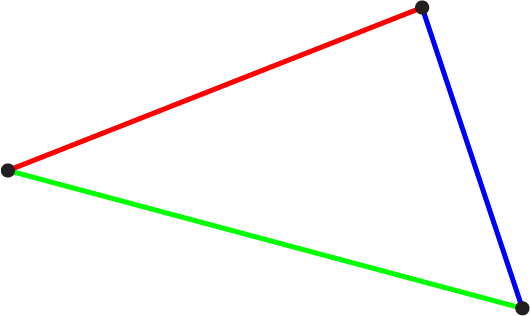
\includegraphics[width=\textwidth]{Images/triangle_logo_thin.png} 
	\end{figure}
}

% Math
\usepackage{amsmath}
\usepackage{amsthm}
\usepackage{amssymb}
\usepackage{amsfonts}
\usepackage{bm}
\usepackage[overload]{empheq} % For braced-style systems of equations.
\usepackage{fix-cm} % To override original LaTeX restrictions on sizes

% Tables
\usepackage{tabularx}
\usepackage{longtable} % Tables that can span several pages
\usepackage{colortbl}

% Algorithms
\usepackage{algorithm}
\usepackage{algorithmicx}
\usepackage{algpseudocodex}
\newcommand*\Let[2]{\State #1 $\gets$ #2}
\newcommand*\AAnd{\textbf{ and }}
\newcommand*\AOr{\textbf{ or }}
\newcommand*\ANot{\textbf{not }}

% Bibliography
\usepackage[colorlinks=true,linkcolor=black,anchorcolor=black,citecolor=black,filecolor=black,menucolor=black,runcolor=black,urlcolor=black]{hyperref} % Adds clickable links at references
\usepackage{cleveref}
\usepackage[square, numbers, sort&compress]{natbib} % Square brackets, citing references with numbers, citations sorted by appearance in the text and compressed
\bibliographystyle{abbrvnat} % You may use a different style adapted to your field

% Other packages
\usepackage{pdfpages} % To include a pdf file
\usepackage{afterpage}
\usepackage{fancyhdr} % For the headers
\fancyhf{}

% Input of configuration file. Do not change config.tex file unless you really know what you are doing. 
% Set the geometric layout of the document
\usepackage{geometry}
\geometry{
  top=3cm,
  left = 1.5cm,
  right = 1.5cm,
  bottom=2cm,
  headheight= 2cm,
  headsep= 0cm,
}
\raggedbottom 

% Create color bluePoli (-> manuale grafica coordinata:  https://www.polimi.it/fileadmin/user_upload/il_Politecnico/grafica-coordinata/2015_05_11_46xy_manuale_grafica_coordinata.pdf)
\definecolor{bluePoli}{cmyk}{0.4,0.1,0,0.4}

% Custom theorem environments
\declaretheoremstyle[
  headfont=\color{bluePoli}\normalfont\bfseries,
  bodyfont=\color{black}\normalfont\itshape,
]{colored}

\captionsetup[figure]{labelfont={color=bluePoli}} % Set colour of the captions
\captionsetup[table]{labelfont={color=bluePoli}} % Set colour of the captions
\captionsetup[algorithm]{labelfont={color=bluePoli}} % Set colour of the captions

\theoremstyle{colored}
\newtheorem{theorem}{Theorem}[section]
\newtheorem{proposition}{Proposition}[section]

% Enhances the features of the standard "table" and "tabular" environments.
\newcommand\T{\rule{0pt}{2.6ex}}
\newcommand\B{\rule[-1.2ex]{0pt}{0pt}}

% Algorithm description
\newcounter{algsubstate}
\renewcommand{\thealgsubstate}{\alph{algsubstate}}
\newenvironment{algsubstates}{
    \setcounter{algsubstate}{0}%
    \renewcommand{\STATE}{%
    \stepcounter{algsubstate}%
    \Statex {\small\thealgsubstate:}\space}
    }{}
    
% Custom theorem environment
\newcolumntype{L}[1]{>{\raggedright\let\newline\\\arraybackslash\hspace{0pt}}m{#1}}
\newcolumntype{C}[1]{>{\centering\let\newline\\\arraybackslash\hspace{0pt}}m{#1}}
\newcolumntype{R}[1]{>{\raggedleft\let\newline\\\arraybackslash\hspace{0pt}}m{#1}}

% Custom itemize environment
\setlist[itemize,1]{label=$\bullet$}
\setlist[itemize,2]{label=$\circ$}
\setlist[itemize,3]{label=$-$}
\setlist{nosep}

% Set separation of columns 
\setlength{\columnsep}{30pt}

% Create command for background pic
\newcommand\BackgroundPic{% Adding background picture
	\put(198,330){
		\parbox[b][\paperheight]{\paperwidth}{%
			\vfill
			\centering
			\transparent{0.4}
			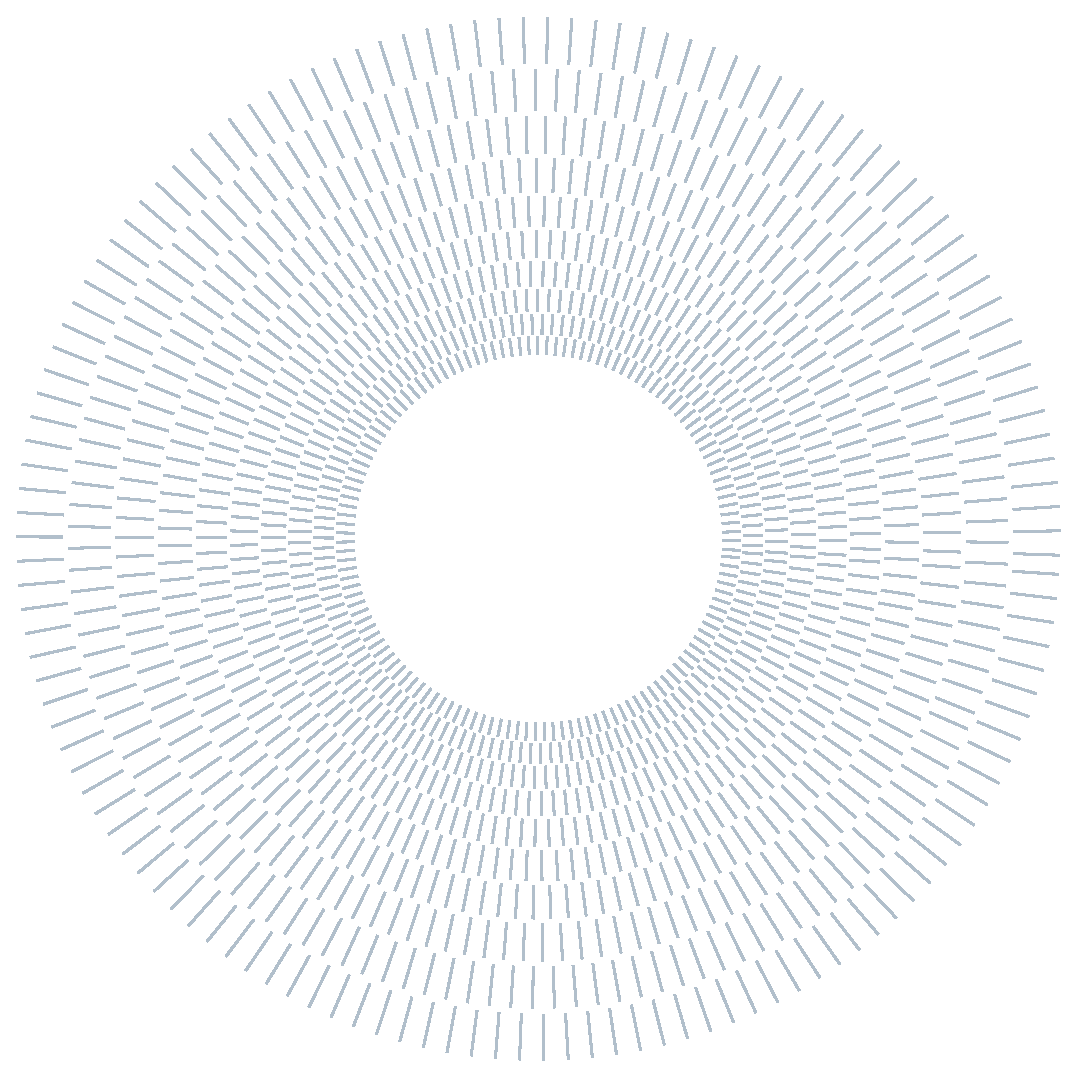
\includegraphics[width=0.7\paperwidth]{raggiera_polimi.eps}%
			\vfill
}}}

% Set indentation
\setlength\parindent{0pt}

% Custom title commands
\titleformat{\section}
{\color{bluePoli}\normalfont\Large\bfseries}
{\color{bluePoli}\thesection.}{1em}{}
\titlespacing*{\section}
{0pt}{2ex}{1ex}

\titleformat{\subsection}
{\color{bluePoli}\normalfont\large\bfseries}
{\color{bluePoli}\thesubsection.}{1em}{}
\titlespacing*{\subsection}
{0pt}{2ex}{1ex}

% Custom headers and footers
\pagestyle{fancy}
\fancyhf{}
      
\fancyfoot{}
\fancyfoot[C]{\thepage} % page
\renewcommand{\headrulewidth}{0mm} % headrule width
\renewcommand{\footrulewidth}{0mm} % footrule width

\makeatletter
\patchcmd{\headrule}{\hrule}{\color{black}\hrule}{}{} % headrule
\patchcmd{\footrule}{\hrule}{\color{black}\hrule}{}{} % footrule
\makeatother

% -> Create the header
\chead[C]{
\centering
\begin{tcolorbox}[arc=0pt, boxrule=0pt, colback=bluePoli!60, width=\textwidth, colupper=white]
    \textsc{\textbf{Executive summary}} \hfill \textsc{\textbf{\author}} 
\end{tcolorbox}
}


% === Start of document ===

\begin{document}
\fancypagestyle{plain}{
\fancyhf{} % Clear all header and footer fields
\fancyhead[R]{\thepage} %RO=right odd, RE=right even
\renewcommand{\headrulewidth}{0pt}
\renewcommand{\footrulewidth}{0pt}}


% === Title page ===
\pagestyle{empty} % No page numbers
\frontmatter % Use roman page numbering style (i, ii, iii, iv...) for the preamble pages

\puttitle{
	title=Ray Distribution Aware Heuristics for Bounding Volume Hierarchies Construction,
	name=Lapo Falcone,
	course=Computer Science and Engineering,
	ID  = 996089,
	advisor= Prof. Marco Gribaudo,
	academicyear={2023-24}
}


% === Preamble ===
\startpreamble
\triangleLogo
\setcounter{page}{1} % Set page counter to 1

% Abstract
\makeatletter
\let\savedchap\@makechapterhead
\def\@makechapterhead{\vspace*{-3cm}\savedchap}
\polimichapter{Abstract}
\let\@makechapterhead\savedchap
\makeatletter
\small
In the last few years, real-time computer graphics have been transitioning from a pipeline based on rasterization to one using ray tracing.
Ray tracing makes it possible to accurately simulate the behavior of light rays, enabling developers of graphics content to reproduce high-fidelity scenes without using a plethora of techniques to mimic light transport.

While ray tracing is widely used for off-line rendering, such as for CGI effects in films or animated movies, the same cannot be stated for on-line applications, such as videogames. The main problem with ray tracing is that simulating light transport is computationally expensive, reason why in recent videogames ray tracing is only used on small portions of the scene or to simulate some effects (such as reflections, shadows, or ambient occlusion).

In order to increase the spread of ray tracing in on-line rendering applications too, research is moving in two macro directions.

The first one is to build GPUs with an architecture more suited for ray tracing, such as the RT cores from Ampere Nvidia GPUs.

The second, but not least important one is to design software optimizations to make ray tracing cheaper.

One of the problems that is ubiquitous in the ray tracing environment is to detect collisions between a ray and the geometry of the scene to render. Given the huge amount of primitives present in modern graphic applications, it is necessary to use a data structure to accelerate the ray collision retrieval process. The state-of-the-art structure is the bounding volume hierarchy (BVH), which hierarchically organizes primitives, making it possible to skip entire sections of the scene that are spatially far away from the ray that is being traced during BVH traversal.

In this work we propose two novel heuristics that work in pairs to build higher-quality BVHs, a data structure to make it possible to use them, and a comparative analysis of their performance in different scenarios.

The first heuristic, called \textbf{projected area heuristic} (PAH), aims at better estimating the amount of rays that hit each node of the BVH by exploiting some artifacts in the ray distribution in the scene, caused by another optimization used in a previous step of the ray tracing pipeline (namely Monte-Carlo importance sampling).

The second one (\textbf{splitting plane facing}) aims at reducing the overlap among nodes of the BVH, consequently reducing the number of intersection tests needed during the BVH traversal phase.

\textbf{Keywords:} Ray tracing, bounding volume hierarchy, BVH
\normalsize

% Abstract in Italian
\makeatletter
\let\savedchap\@makechapterhead
\def\@makechapterhead{\vspace*{-3cm}\savedchap}
\polimichapter{Abstract in Lingua Italiana}
\let\@makechapterhead\savedchap
\makeatletter
\small
Abstract Italiano
\\
\\
\textbf{Parole chiave:} Ray tracing, bounding volume hierarchy, BVH
\normalsize


% === Table of contents ===
\thispagestyle{empty}
\tableofcontents % Table of contents 
\thispagestyle{empty}
\cleardoublepage

\addtocontents{toc}{\vspace{2em}} % Add a gap in the Contents, for aesthetics
\mainmatter % Begin numeric (1,2,3...) page numbering

% Add logo to page numbers
\AddToShipoutPicture{%
	\put(\textwidth+58,\textheight+88){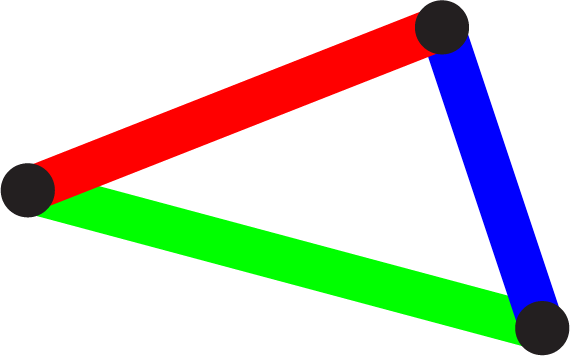
\includegraphics[scale=0.06]{Images/triangle_logo.png}}
}

% === Intro ===
\chapter*{Introduction}
\large \textbf{Why ray tracing?} \normalsize\\
In the field of computer graphics, we refer to ray tracing as a family of rendering algorithms that simulate light transport in order to transition from a mathematical representation of a scene to an image on the screen. 

TODO same in chapter 1
Conceptually ray tracing is an extremely straightforward technique, that can be summarized in a few steps:
\begin{enumerate}
\item Generate a ray of light from a light source;
\item Find out the first object the ray intersects;
\item Compute how much energy is absorbed by the material of the object;
\item Modify the direction of the ray based on the material of the object (for example it may be reflected or refracted);
\item Repeat from 2. until the ray hits the camera;
\item Color the pixel of the camera hit by the ray based on the energy of the ray.
\end{enumerate}

\begin{figure}[H]
    \centering
    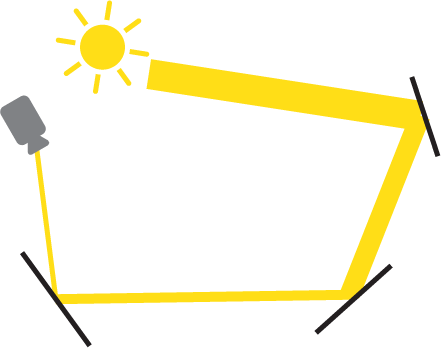
\includegraphics[scale=0.4]{Images/ray_tracing_simple.png}
    \caption{The width of the yellow ray represents the amount of energy carried. After each intersection some energy is absorbed.}
    \label{fig:ray_tracing_simple}
\end{figure}

Since ray tracing mimics the behavior of light in the real world, the technique can be directly used to simulate complex light effects that would require the use of ad-hoc and approximate methods if we use other rendering algorithms, such as the widely spread rasterization pipeline.

To give an intuition of how the ad-hoc methods can be convoluted and produce worse results, we summarize one of the most intuitive ones used to generate shadows, called shadow mapping. A shadow map is the projection of the scene from the point of view of a point light source, saved in a texture where each pixel stores the distance from the light source to the projected point. When the scene is projected by the main camera, each visible point is transformed into the coordinate system of the shadow map via matrix multiplication, and is then compared to the point stored in the corresponding pixel of the shadow map. If the point of the shadow map is closer to the light source than the corresponding point projected by the main camera, we deduce that such a point is not visible from the point of view of the light source and, therefore, is in shadow. This specific technique is correct only with point lights, and must be adjusted in case translucent objects are present in the scene.

With ray tracing shadows are natively generated since, if a point is in shadow, no light ray starting from it will hit the camera pixels. Moreover, in principle, it works with any kind of light, not only point lights, and thus produces higher-quality shadows, since no approximations must be made.

\large \textbf{We need optimizations} \normalsize\\
Until now we briefly highlighted the strong points of ray tracing, and greatly simplified it. The main issue with ray tracing is that it is computationally expensive to simulate light transport. Of course, it is impossible to track the path of every photon emitted by a light source, therefore, even in ray tracing algorithms, some approximations must be made. The nature of the approximations depends on the specific ray tracing algorithm used. For example, in many techniques falling under the name of \textit{backward ray tracing} \footnote{In some literature the term \textit{backward ray tracing} can also refer to the opposite family of algorithms, since the first ray tracing methods were indeed backward.}, rays don't start from the light sources, but from the camera, and gain energy when they hit a light source. At this point the path described by the ray is followed backward and the energy hitting the pixel of the camera is computed. In this way the number of rays is greatly reduced, because all the rays hit the camera, therefore none is wasted. On the other hand, some phenomena (such as caustics) cannot be realistically simulated.

From this point on we will consider the scenario where rays are traced backwards.

One optimization that is foundational to modern ray tracing and relevant to our work, is the use of the \textbf{Monte-Carlo} integration method, and, in particular, a variance reduction technique called \textbf{importance sampling}. We will introduce the concept in this section in an oversimplified way, and then explain it from a mathematical standpoint in \ref{TODO}.

When a ray hits a point on a surface, it may bounce in any direction, based on the material. The most intuitive bounce is a perfect reflection, but, since at a microscopic level surfaces are never perfectly planar, it is possible for the incoming ray to bounce in any direction. This phenomenon is described in a probabilistic way by the bidirectional reflective distribution function (BRDF). Each material is described by a BRDF, and each BRDF makes it more likely for a ray coming from a certain direction to bounce to another range of directions (for example, for a perfectly reflective material, the BRDF will return a probability of 1 for a ray to bounce to the perfect reflection direction).

\begin{figure}[H]
    \centering
    \subfloat[Perfectly reflective surface.]{
        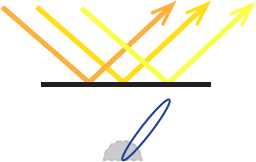
\includegraphics[scale=0.45]{Images/reflective_brdf.png}
		}
		\qquad
	\subfloat[Non-reflective surface.]{
        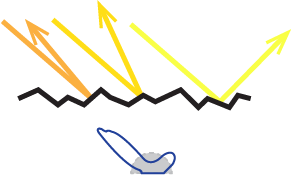
\includegraphics[scale=0.45]{Images/non_reflective_brdf.png}
    }
	\caption{In figure (a) all the rays coming from a direction are reflected towards the same direction. In (b), instead, the surface is microscopically rough, 2 rays coming from the same direction could bounce to 2 very different directions. Under each figure there is the corresponding graph of its BRDF.} 
    \label{fig:surfaces_reflectiveness}
\end{figure}

Therefore, if we wanted to accurately simulate the light behavior after a ray hits a material, and compute how much light is reflected towards a specific direction (the one of the incoming ray), we would need to send a probe ray to every direction of the hemisphere centered on the hit point, get back the light energy carried by each probe ray, and compute an average based on the probability of each probe ray given by the BRDF. In short, we would need to integrate the light energy function over the hemisphere. This exact same process would then need to be replicated when each probe ray hits an object, recursively, until each ray in the scene hits a light source or gets completely absorbed.

This process, of course, is not feasible, but it can be approximated by the Monte-Carlo method with fewer samples. The idea is that, instead of probing each direction of the hemisphere with a ray, we probe just a small number (often just one) of directions. In most cases the estimate of the light incoming to the point will not be accurate, but, granted that there is a high enough number of incoming rays hitting the neighborhood of the point, the incoming light average will indeed be accurate.

In order to get the most out of the probe rays we cast out of a hemisphere, we would like to send them in directions that contribute the most to the final value we are trying to calculate, namely the light reflected toward the direction of the incoming ray. This is the base concept behind importance sampling. In ray tracing there are two common ways to achieve this:
\begin{description}
\item[BRDF sampling] Probe rays are cast in directions where the BRDF returns a high weight. In this way the energy the probe rays carry is multiplied by a value close to 1; on the other hand, the energy can be a low value.
\item[Light sampling] Probe rays are cast directly towards light sources. In this way they will likely carry a lot of energy (unless an obstacle is hit), but the BRDF weight they will be multiplied with may be small.
\end{description}
It is even possible to combine the two techniques with a method called multiple importance sampling (MIS).

The use of importance sampling generates artifacts in the ray distribution on the scene. Rays' directions will no longer be distributed uniformly, but, due to light sampling, more rays will tend to go towards light sources.

\large \textbf{Rays intersections} \normalsize\\
One of the problems that is common to all the algorithms of the ray tracing family is to find the intersection between a ray and the geometry of the scene.

The objects in the scene are usually meshes, which are a collection of geometric primitives. In many real-world scenarios, primitives are simple triangles, described by 3 vertices. Therefore, the problem of intersecting a ray with the scene is reduced to the problem of intersecting a ray with a collection of triangles.

Given an algorithm to find out if a ray hits a triangle in \ref{sec:ray_triangle_intersection}, the naive way of retrieving the closer triangle hit by a ray would be to perform the ray-triangle test on all the triangles present in the scene. Such an algorithm has a complexity of $\mathcal{O}(n\cdot m)$ where $n$ is the number of triangles and $m$ the number of rays.

Acceleration structures have been developed to speed up the process. The state-of-the-art acceleration structure used in ray tracing is the \textbf{bounding volume hierarchy} (BVH).

In summary, a BVH is a binary tree\footnote{Technically it can be a tree with any breadth, but binary trees are the most common ones.} where each node wraps some of the triangles in the scene in a bounding volume, usually an axis-aligned bounding box (AABB). Given a node $A$ wrapping the triangles in the set $T_A$, the two children of $A$, called $B$ and $C$ wrap the triangles in the sets $T_B$ and $T_C$ such that $T_B \cup T_C = T_A$. Thanks to this structure, if a ray doesn't intersect a bounding volume, we deduce that it will not intersect any of the triangles contained in the bounding volume too, making it possible to discard them without having to perform any additional intersection test. This means that, if the BVH is balanced, the the complexity to find an intersection between a ray and the scene is $\mathcal{O}(log_2(n) \cdot m)$.

\begin{figure}[H]
    \centering
    
\includegraphics[scale=0.4]{Images/TODO.png}
    \caption{A 2-dimensional BVH.}
    \label{fig:bvh_2d}
\end{figure}

Given the definition and the advantages of a BVH over the naive algorithm, we now have to build a BVH starting from the primitives in the scene.
Building the optimal BVH is an NP-complete problem since, for each level of the BVH, we would have to try all the possible ways to subdivide the triangles into 2 AABBs, recursively, until all the branches are leaves; then measure the quality of the BVHs and take the best one.

In a real-world scenario a greedy algorithm is used instead, where, at each level, some of the possible ways to subdivide the triangles are tried, and the best one with reference to a cost metric function is greedily taken. This means that, even if in the next level it is found out that the split in a previous level was not optimal, the algorithm proceeds without changing the previous decision.

The quality of the trees built with such an algorithm depends on many factors, but two of the most relevant ones are the cost function and how the algorithm tries to split the triangles at each level.

\large \textbf{The surface area heuristic} \normalsize\\
The vast majority of the state-of-the-art algorithms to build BVHs uses the \textbf{surface area heuristic (SAH)} as cost metric. SAH is extremely simple and fast: the cost of a node $K$ is proportional to the probability that a random ray intersects the node $p(hit\:K)$, and the number of primitives the node contains $\#T_K$:
$$SAH(K) = p(hit\:K) \cdot \#T_K$$

The probability that a node is hit by a random ray is proportional to its area: $p(hit\:K) = \frac{A_K}{A_tot}$ where $A_tot$ is the area of the AABB enclosing the whole scene.
Computing the area of an AABB is trivial.

SAH is based on three hypotheses:
\begin{enumerate}
	\item All the rays hit AABB enclosing the whole scene.
	\item All the rays start from outside the scene.
	\item Rays are distributed in a uniform random way on their 6-dimensional space (3 dimensions for the position of their origin and 3 dimensions for their direction).
\end{enumerate}

None of these hypotheses is satisfied in a real-world scenario, and, in particular, we will focus on the third one.

As we noted above, due to the use of importance sampling, rays are not distributed uniformly in the scene. In particular, due to light sampling, in proximity of light sources, rays have directions pointing towards the light source. Based on the light source type, we have different types of ray distributions, as it is possible to appreciate in the images below.

\begin{figure}[H]
    \centering
    \subfloat[Point light generated distribution]{
        
\includegraphics[scale=0.25]{Images/TODO.png}
		}
		\qquad
	\subfloat[Area light generated distribution]{
        
\includegraphics[scale=0.25]{Images/TODO.png}
    }
	\caption{The ray distributions generated by point and area lights.}
    \label{fig:generated_distributions}
\end{figure}

Area lights tend to generate regions where rays are parallel. This means that we can better estimate the probability that a ray intersects an AABB by computing its projected area on the plane perpendicular to the bundle of rays, instead of the surface area of the AABB. Such a projected area can be computed with an orthographic projection.

Point lights, instead, tend to generate a bundle of lines passing through a point, and therefore the projected area can be computed with a perspective projection.

In this work we aim to show how this way of computing the cost function for the construction of a BVH can produce higher quality BVHs in some situations. We named this novel approach as \textbf{projected area heuristic (PAH)}.


\chapter{Background Theory}
\label{ch:background_theory}
In this chapter we will summarize the background knowledge needed to fully comprehend this work.

In section \ref{sec:ray_tracing_principles} we will introduce ray tracing in simple terms, and list some of its advantages, disadvantages and its today's applications.

In section \ref{sec:monte_carlo_and_variance_reduction_techniques} we will analyze from a mathematical standpoint how the most used ray tracing algorithms work.

Last, in section \ref{sec:ray_tracing_acceleration_structures}, we will describe the state-of-the-art acceleration structure to make a fundamental ray tracing procedure (ray-scene intersection) faster.

\section{Ray Tracing Principles} \label{sec:ray_tracing_principles}
\subsection{High Level Overview}
Ray tracing is a family of rendering algorithms that is used in computer graphics to transition from a mathematical representation of a scene, to an image on the screen.

Conceptually ray tracing is an extremely straightforward technique, that can be summarized in a few steps:
\begin{enumerate}
\item Generate a ray of light from a light source;
\item Find out the first object the ray intersects;
\item Compute how much energy is absorbed by the material of the object;
\item Modify the direction of the ray based on the material of the object (for example it may be reflected or refracted);
\item Repeat from 2. until the ray hits the camera or loses all its energy;
\item Color the pixel of the camera hit by the ray based on the energy of the ray.
\end{enumerate}

Ray tracing aims to mimic the real-world behavior of light, and for this reason it can be directly employed to simulate any light effect, starting from the simplest ones, such as perfect reflections and shadows, going towards the most complex ones, such as global illumination and caustics. Some of the most accurate ray tracing algorithms can even simulate quantum effects of light \cite{quantum_ray_tracing}.

Since ray tracing natively simulates light, it can produce extremely realistic images, without resorting to ad-hoc techniques used to approximate light phenomena in other rendering algorithms, such as the widely spread rasterization pipeline.

To give an intuition of how the ad-hoc methods can be convoluted and produce worse results, we summarize one of the simplest ones used to generate shadows, called shadow mapping \cite{shadow_maps}. A shadow map is the projection of the scene from the point of view of a point light source, saved in a texture where each pixel stores the distance from the light source to the projected point. When the scene is projected by the main camera, each visible point is transformed into the coordinate system of the shadow map via matrix multiplication (figure \ref{fig:shadow_map}). The point in the new coordinate system is then compared to the point stored in the corresponding pixel of the shadow map. If the point of the shadow map is closer to the light source than the corresponding point projected by the main camera, we deduce that such a point is not visible from the point of view of the light source and, therefore, is in shadow. This specific technique is correct only with point lights, and must be adjusted in case translucent objects are present in the scene.

With ray tracing shadows are natively generated since, if a point is in shadow, no light ray starting from it will hit the camera pixels. Moreover, in principle, it works with any kind of light, not only point lights, and thus produces higher-quality shadows, since no approximations must be made.

\begin{figure}[]
    \centering
    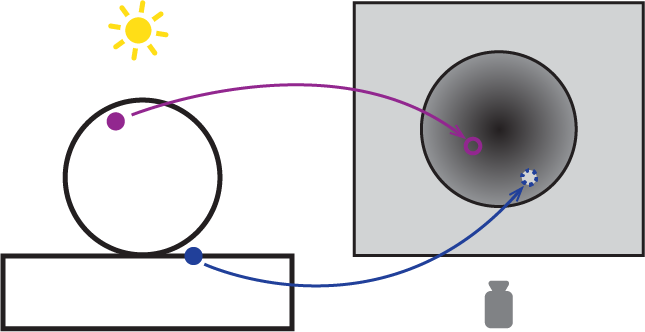
\includegraphics[scale=0.6]{Images/shadow_map.png}
    \caption{The first figure is from the main camera PoV, the second one from the light source PoV. The second figure represents depth: the closer a point is to the light source, the darker. The blue point is in shadow, because the corresponding point in the shadow map is further away than the stored depth.}
    \label{fig:shadow_map}
\end{figure}

\subsection{Use Cases}
Due to the highly realistic images ray tracing algorithms can produce, the technique has found a lot of success in many applications. We can subdivide the use cases into two macro-categories: real-time ray tracing and production ray tracing.

The most prominent use of the second category is in movies. CGI effects and animated films are almost always produced by using ray tracing \cite{path_tracing_movies}, in particular a very accurate algorithm called bi-directional path tracing \cite{bidirectional_path_tracing}. In the first category we can find videogames.

The main difference between real-time and production ray tracing lies in the time constraints for producing a frame. In production ray tracing producing a frame can take a long time, even in the order of magnitude of days. Whereas, in real-time ray tracing, a frame must be produced every $33$ms to achieve $30$ frames per second (fps), and every $16.5$ms to achieve $60$ fps, which can be considered today's standard by many PC videogames.

This starking difference makes it so that different techniques must be used depending on the scenario. In real-time ray tracing many approximations must be introduced in order to stay within the frame time budget, whereas in production ray tracing more accurate algorithms can be used, since time constraints are loose. Our work can benefit both categories, since the methods we will introduce can make ray tracing faster, in some situations, without introducing approximations.

\subsection{Optimizations Overview} \label{ssec:optimizations_overview}
Until now we briefly highlighted the strong points of ray tracing, and greatly simplified it. The main issue with ray tracing is that it is computationally expensive to simulate light transport in a convincing way. The reason lies in the rendering equation, and will be explained in section \ref{sec:monte_carlo_and_variance_reduction_techniques}.

In order to make ray tracing usable in the real world, the industry moved in two directions:
\begin{description}
	\item [Hardware accelerators] GPU vendors, in particular Nvidia, started creating GPUs with specialized cores for ray tracing. These cores have a memory layout that makes it faster to find a ray-triangle intersection. An example of this can be the RT cores from Turing Nvidia GPUs \cite{rt_cores}.
	\item [Software optimizations] Software developers introduced new algorithms to improve the performance of a specific part of the ray tracing pipeline. These algorithms can vary a lot in complexity and results. One of the most common optimizations for real-time ray tracing is to use ray tracing only for some light effects (such as shadows or reflections), while using rasterization for most of the scene.
\end{description}

Software optimizations can, in turn, be subdivided into two big families.

Some optimizations aim at improving the time needed to detect the first intersection of a ray with the scene. These optimizations don't alter the quality of the rendered scene. We will diffusely talk about these optimizations in section \ref{sec:ray_tracing_acceleration_structures}, and this work can be placed into this family.

The other family comprehends optimizations aimed at reducing the number of rays needed to produce a visually acceptable image. This work, while being part of the first family of optimizations, has its foundations in an artifact in the ray distribution in the scene caused by an optimization of this second family. This technique is called importance sampling, and will be discussed in section \ref{sec:monte_carlo_and_variance_reduction_techniques}.

\subsection{Backward Ray Tracing}
Before going to the next section, it is important to introduce the concept of backward ray tracing\footnote{In some literature the term \textit{backward ray tracing} can also refer to the opposite family of algorithms, since the first ray tracing methods were indeed backward.}. 

In backward ray tracing light rays don't start from light sources, but from the eye position. Starting from the eye, each ray will then hit a fictitious plane placed in front of the eye (the near plane), similar to what happens in a pinhole camera \cite{pinhole_camera}. The near plane can be subdivided into discrete units displaced in a regular grid, which we will consider the pixels of the final image. Each ray is therefore associated with the pixel it hits, and will contribute to its final color.

\begin{figure}[H]
    \centering
    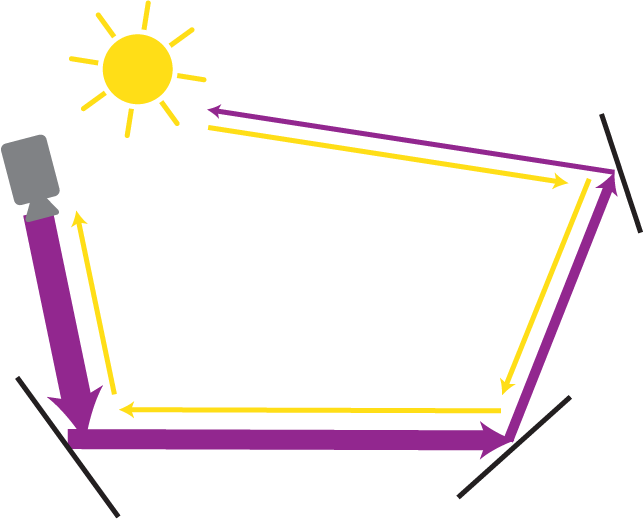
\includegraphics[width=\textwidth*\real{0.6}]{Images/backward_ray_tracing.png}
    \caption{How rays are cast in backward ray tracing.}
    \label{fig:pinhole_camera}
\end{figure}

The rays starting from the camera will hit the scene and bounce around. At each bounce a ray loses a fraction of its energy (unless the surface is perfectly reflective), until either it gets completely absorbed, or it hits a light source. In the case a ray hits a light source, we already know how much of its energy will be lost due to intersections with objects, therefore we can immediately compute the color of the pixel associated with the ray (as if we followed that same ray's path backward). If a ray never hits a light source, it will not contribute to the color of its associated pixel, because it never gain energy.

A way of looking at this algorithm is to think we are tracing \textit{importons}, which can be considered the dual concept of \textit{photons} \cite{importons}. Thanks to the light reciprocity principle \cite{light_reciprocity}, which states that light transmits in the same way in both directions, tracing photons or importons is equivalent.

The advantage of backward ray tracing is that, with a limited budget of rays we can cast, it is more efficient than forward ray tracing. Indeed, in forward ray tracing it is possible a ray never hits the camera, in which case it would be wasted. In backward ray tracing all the rays hit the camera by definition, thus none is wasted.

Of course, if a ray starting from the camera never hits a light source, it could be considered wasted, but some techniques that will be described in section \ref{sec:monte_carlo_and_variance_reduction_techniques} make it more likely for a ray to hit a light source in its path.

From this point on, we will consider the scenario where rays are traced backwards.

\section{Monte-Carlo and Variance Reduction Techniques} \label{sec:monte_carlo_and_variance_reduction_techniques}
In this section we will analyze the mathematical foundations of ray tracing, namely the Kajiya's rendering equation. Then we will present a statistical method to resolve the integrals appearing in the rendering equation, called Monte-Carlo. Finally, we will discuss a variance reduction technique, importance sampling, that can be used to obtain better approximations from the Monte-Carlo method, without making it more expensive. We will see how this technique generates artifacts in the ray distribution in the scene, which is one of the hypotheses of our thesis.

\subsection{Kajiya's Rendering Equation}
$$
L_o(\bar{x},\bar{\omega}_o) = L_e(\bar{x}, \bar{\omega}_o) + \int_\Omega BRDF(\bar{x}, \bar{\omega}_i, \bar{\omega}_o) \cdot \cos(\bar{n}, \bar{\omega}_i) \cdot L_i(\bar{x}, \bar{\omega}_i) d\bar{\omega}_i
$$

This equation, developed by James T. Kajiya in 1986 \cite{rendering_equation}, can be used to calculate the amount of light \textit{generated} by a point $\bar{x}$ towards a direction $\bar{\omega}_o$. As we will see in the next paragraphs, with the term \textit{generated} we refer to the sum of the light emitted by the point, and the light reflected by it. In order to compute the \textit{generated} light we need to know these variables:
\begin{itemize}
	\item $L_e(\bar{x}, \bar{\omega}_o)$ The light emitted by the point $\bar{x}$ towards a direction $\bar{\omega}_o$.
	\item $BRDF$ The bidirectional reflectance distribution function of the material at point $\bar{x}$.
	\item $\bar{n}$ The normal to the surface at point $\bar{x}$.
	\item $L_i(\bar{x}, \bar{\omega}_i)$ The light incoming to $\bar{x}$ from a generic direction $\bar{\omega}_i$ on the hemisphere $\Omega$ orientated toward $\bar{n}$.
\end{itemize}

The equation can be divided into two parts:

The first part describes the light emitted $L_e(\bar{x}, \bar{\omega}_o)$, and it is 0 unless the point is a light source. Depending on the light source type, it can assume a uniform value in each direction (point light), a value only in one hemisphere (a plane area light), or a specific value based on the direction, usually controlled by a function (such as in spotlight). In any case the emitted light value is known by the definition of the light source in the scene, therefore can be easily plugged into the equation.

\begin{figure}[H]
    \centering
    \subfloat[Point light]{
        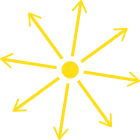
\includegraphics[width=\textwidth*\real{0.25}]{Images/point_light.png}
	}
	\qquad
	\subfloat[Plane area light]{
        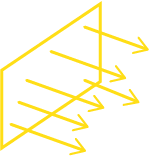
\includegraphics[width=\textwidth*\real{0.25}]{Images/plane_light.png} 
    }
	\qquad
	\subfloat[Spotlight]{
        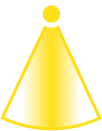
\includegraphics[width=\textwidth*\real{0.22}]{Images/spot_light.png}
    }
	\caption{Three possible types of light sources.}
    \label{fig:light_sources}
\end{figure}

The second part of the equation presents an integral, and represents the light reflected by the material of the point towards the direction $\bar{\omega}_o$. In simple words, this second term tells us that, in order to compute the reflected light, we have to know, first, how much light is incoming to the point from all the directions in the hemisphere $\Omega$. And second, the properties of the material, summarized in the $BRDF$ \cite{brdf}. The $BRDF$ tells us how much of the incoming light is reflected towards the direction $\bar{\omega}_o$. 

\begin{figure}[H]
    \centering
    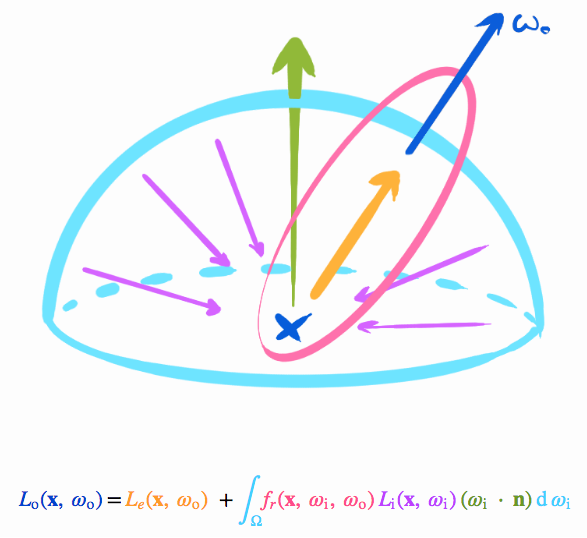
\includegraphics[width=\textwidth*\real{0.5}]{Images/kajiya_visual.png}
    \caption{A visual representation of the Kajiya rendering equation from \cite{kajiya_equation_drawing}.}
    \label{fig:rendering_equation}
\end{figure}

The term $\cos(\bar{n}, \bar{\omega}_i)$ is called geometry term, and reflects a core property of light, independent of the $BRDF$. Indeed, based on the angle a beam of light intersects a surface, the beam of light will enlighten a smaller or bigger area of the surface. The smallest surface is illuminated when the direction of the beam of light and the normal to the surface are parallel. Since the energy carried by the beam of light is constant, we can deduce that, the bigger the enlightened surface, the lower the energy per area unit. In particular, if we let $L$ be the energy of the beam and $\alpha$ the angle between the beam direction and the normal, then the energy received per area unit equals to $L\cdot \cos(\alpha)$. 

\begin{figure}[H]
    \centering
    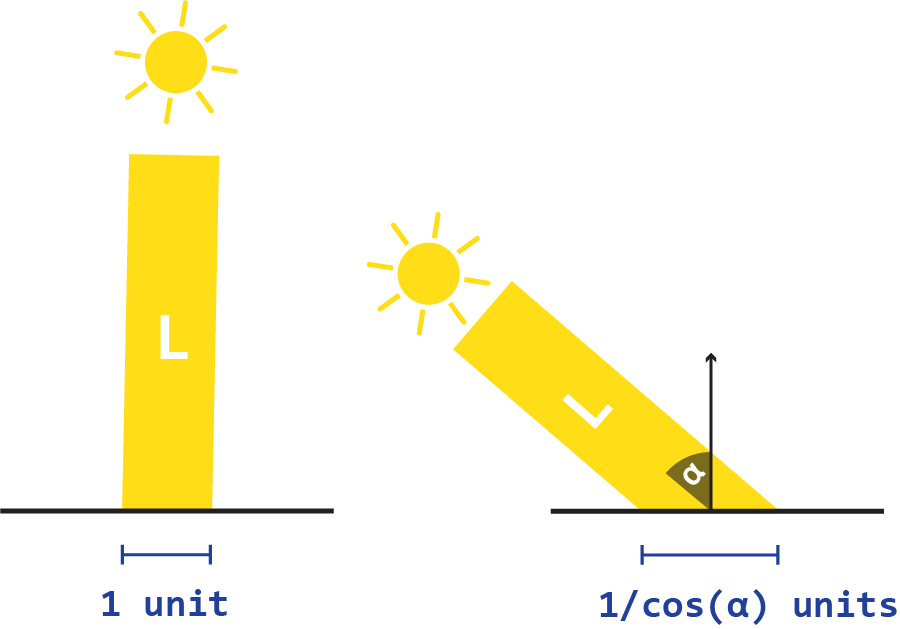
\includegraphics[width=\textwidth*\real{0.7}]{Images/geometry_term.png}
    \caption{The geometry term.}
    \label{fig:geometry_term}
\end{figure}

When we compute the integral term of the rendering equation, the BRDF is known by definition, and the geometry term is a simple cosine. On the other hand, we almost never have an analytical form of the $L_i$ term, and it is indeed this specific part of the equation what really makes ray tracing expensive.

In order to compute the $L_i$ term for one specific direction $\overline{\omega_{\tilde{i}}}$, we can cast a probe ray $R_1$ from point $\overline{x}$ toward $\overline{\omega_{\tilde{i}}}$. The probe ray will hit another point $\overline{y}$. Now, since we want to compute how much light $R_1$ is carrying towards $\overline{x}$, we have to resolve the rendering equation at point $\overline{y}$ and with outgoing direction $-\overline{\omega_{\tilde{i}}}$, namely $L_o(\overline{y}, -\overline{\omega_{\tilde{i}}})$. In other words, the light incoming to one point from one direction, equals the light outgoing from a second point towards the same direction (with inverted sign). This recursive pattern is usually ended after a certain number of bounces (when we can consider that the ray is carrying an infinitesimal amount of energy), or when a probe ray hits a light source (where the generated light is only influenced by the emitted light term of the rendering equation).

\begin{figure}[H]
    \centering
    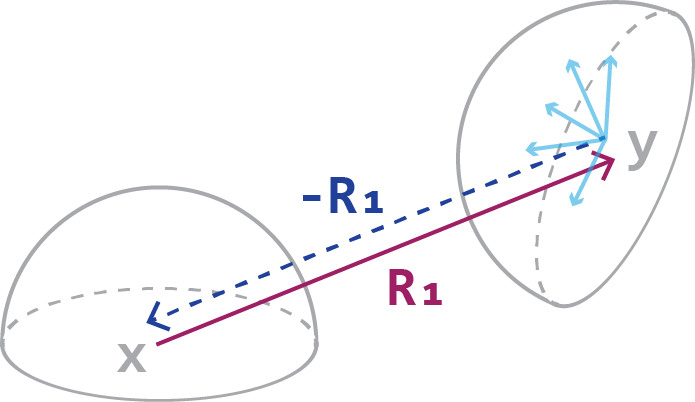
\includegraphics[width=\textwidth*\real{0.5}]{Images/kajiya_recursive.png}
    \caption{Recursiveness of the integral term of the Kajiya rendering equation.}
    \label{fig:kajiya_recursiveness}
\end{figure}

The process we've just described only returns the amount of light incoming to $\overline{x}$ from an arbitrary direction $\overline{\omega_{\tilde{i}}}$. But, as we can see, in the rendering equation an integral over the hemisphere $\Omega$ is present, therefore, in order to have a mathematically correct result, we would need to cast an infinite amount of probe rays. This is not feasible, and leads us to the Monte-Carlo method.

\subsection{Monte-Carlo Integration} 
In this section we will provide an intuition of the Monte-Carlo integration method, and its basic mathematical foundations necessary to fully understand this work.

Monte-Carlo integration \cite{monte_carlo_integration} is a method by which it is possible to compute the numerical integral of a function by using random samples.
Given a one-dimensional positive integrable function $f$, we can interpret its definite integral in the $[a,b]$ interval as the area between the curve and the x-axis.
Now, if we select a random point $k_0$ uniformly in the $[a,b]$ interval, we can compute the area $A_r$ of the rectangle with side $\overline{ab}$ and height $f(k_0)$ as $\overline{ab} \cdot f(k_0)$. We can interpret it as a very rough approximation of the area under the function, which, by definition, is equal to the definite integral value. If we repeat this process $N$ times and compute the average of the various $A_r$s, we'll usually get a better estimate of the area under the function, because sometimes we will underestimate its value, and sometimes we will overestimate it.

\begin{figure}[H]
    \centering
    \subfloat[Area approximation with one sample.]{
        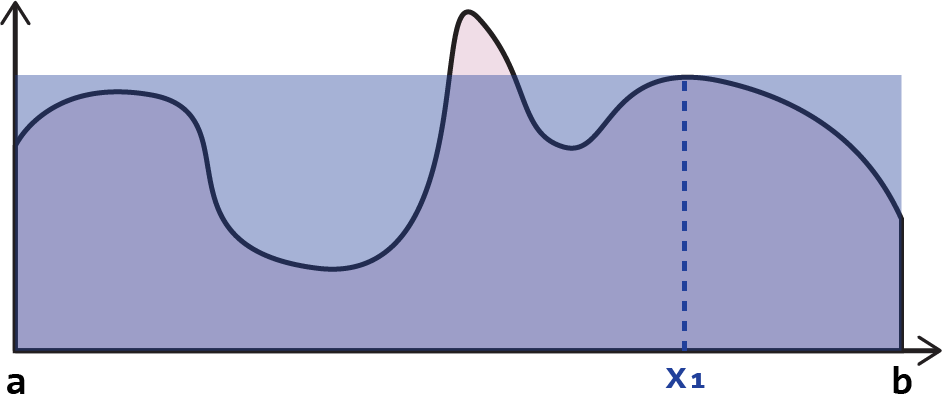
\includegraphics[width=\textwidth*\real{0.65}]{Images/monte_carlo_area_1x.png}
	}
	\qquad
	\subfloat[Area approximation with 4 samples]{
        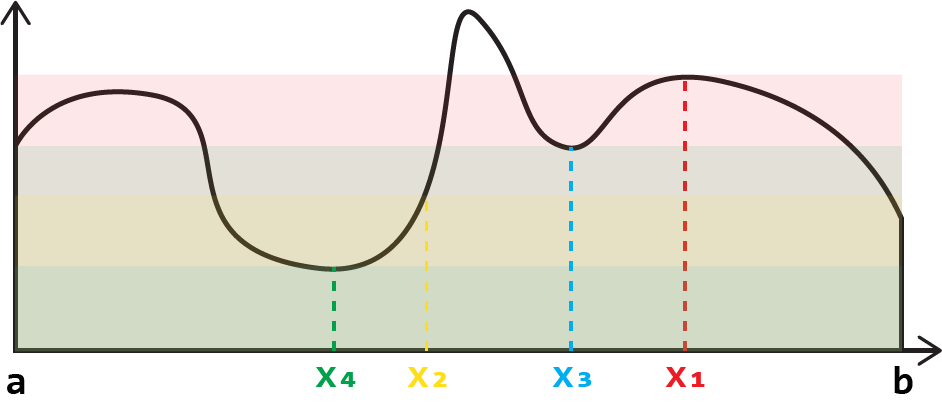
\includegraphics[width=\textwidth*\real{0.65}]{Images/monte_carlo_area_4x.png}
    }
	\caption{Monte-Carlo area approximation. When we hame many samples, sometimes the area will be overestimated, some other times underestimated.}
    \label{fig:monte_carlo_area_approximation}
\end{figure}

We can formalize this process with this formula, where $X_i \sim \frac{1}{b-a}$ is a uniform random variable in the $[a,b]$ interval. 

$$\langle F^N \rangle = \frac{1}{N}\cdot (b-a)\cdot\sum_{i=0}^{N-1}\textit{f}(X_i)$$

$\langle F^N \rangle$ is referred to as the basic Monte-Carlo estimator \cite{monte_carlo_estimators_veach} \cite{monte_carlo_estimators_scratchapixel}. The Monte-Carlo estimator, being a linear combination of random variables, is a random variable itself. Monte-Carlo theory states that the expected value of the Monte-Carlo estimator equals the definite integral of $f$. Below we prove this statement:

\begin{subequations}
	\begin{align*}
		E[\langle F^N \rangle] &= E[(b-a)\cdot \frac{1}{N}\sum_{i=0}^{N-1}\textit{f}(X_i)] \\
		&= (b-a)\cdot \frac{1}{N}\cdot\sum_{i=0}^{N-1} E[\textit{f}(X_i)] \\
		&= (b-a)\cdot \frac{1}{N}\cdot\sum_{i=0}^{N-1}\int_{a}^{b}\textit{f}(x) \cdot \frac{1}{b-a} dx \\
		&= \frac{1}{N}\cdot\sum_{i=0}^{N-1}\int_{a}^{b}\textit{f}(x) dx \\
		&= \int_{a}^{b}\textit{f}(x) dx
	\end{align*}
\end{subequations}

In order to go from line 2 to line 3, it is important to remember the law of the uncounscious statistician (LOTUS) \cite{lotus}, where $p$ is the probability density function of the random variable $X$:
$$E[\textit{f}(X)] = \int_{\Omega}\textit{f}(x)\cdot p(x) dx$$ 

The LOTUS is easier to understand in its discrete case, where $E[\textit{f}(x)] = \sum\textit{f}(x)\cdot p(x)$. This can, for example, be visualized to compute the expected value of a fair die throw: each side has $\frac{1}{6}$ chances of appearing, therefore the expected value equals: $\frac{1}{6} \cdot 1 + \frac{1}{6} \cdot 2 + \frac{1}{6} \cdot 3 + \frac{1}{6} \cdot 4 + \frac{1}{6} \cdot 5 + \frac{1}{6} \cdot 6 = 3.5$. If the die was unfair and, for example, $6$ has a probability to appear of $\frac{1}{2}$, and the remaining 5 sides have a probability of $\frac{1}{10}$ then the expected value would be skewed towards high numbers: $\frac{1}{10} \cdot 1 + \frac{1}{10} \cdot 2 + \frac{1}{10} \cdot 3 + \frac{1}{10} \cdot 4 + \frac{1}{10} \cdot 5 + \frac{1}{2} \cdot 6 = 4.5$. 

Monte-Carlo integration can be used even if the random variable $X_i$ follows a non-uniform distribution. Let the probability density function (PDF) of $X_i$ be $p$, then the Monte-Carlo estimator can be written as \cite{monte_carlo_estimators_veach} \cite{monte_carlo_estimators_scratchapixel}:

$$\langle F^N \rangle = \frac{1}{N}\cdot\sum_{i=0}^{N-1}\frac{\textit{f}(X_i)}{p(X_i)}$$

We can prove the formula with an analogous proof to the one above (this time the integration domain is $\Omega$): 

\begin{subequations}
	\begin{align*}
		E[\langle F^N \rangle] &= E[\frac{1}{N}\cdot\sum_{i=0}^{N-1}\frac{\textit{f}(X_i)}{p(X_i)}] \\
		&= \frac{1}{N}\cdot\sum_{i=0}^{N-1}E[\frac{\textit{f}(X_i)}{p(X_i)}] \\
		&= \frac{1}{N}\cdot\sum_{i=0}^{N-1}\int_{\Omega}\frac{\textit{f}(x)}{p(x)} \cdot p(x) dx \\
		&= \frac{1}{N}\cdot\sum_{i=0}^{N-1}\int_{\Omega}\textit{f}(x) dx \\
		&= \int_{\Omega}\textit{f}(x) dx
	\end{align*}
\end{subequations}

Monte-Carlo integration enjoys some important properties that make it suitable to solve many problems concerning integrals, among which the rendering equation.

First, the Monte-Carlo estimator $\langle F^N \rangle$ is consistent, meaning that, as $N$ tends to infinity, the estimator converges to a value.

Moreover, it is also unbiased, therefore the value it converges to is the value of the definite integral of the function Monte-Carlo is estimating \cite{monte_carlo_properties}. 

Compared to other integration techniques, such as Riemann sum, Monte-Carlo doesn't suffer from the \textit{curse of dimensionality} \cite{curse_of_dimensionality}. \textit{Curse of dimensionality} means that the complexity of the algorithm to compute the integral grows exponentially as the number of its dimensions increases: $\mathcal{O}(k^d)$. This is particularly relevant in our case, since we are working in a 3-dimensional domain.

We can now calculate the variance and standard deviation of the Monte-Carlo estimator $\sigma[\langle F^N \rangle]$ in order to show the convergence rate of this technique. Here we use the random variable $Y$ as  $\frac{\textit{f}(X)}{p(X)}$:

\begin{subequations}
	\begin{align*}
		\sigma[\langle F^N \rangle] &= \sqrt{V[\langle F^N \rangle]} \\
		&= \sqrt{V[\frac{1}{N}\cdot \sum_{i=0}^{N-1}Y_i]} \\
		&= \sqrt{\frac{1}{N^2}\cdot V[\sum_{i=0}^{N-1}Y_i]} \\
		&= \sqrt{\frac{1}{N^2}\cdot \sum_{i=1}^{N-1}V[Y_i]} \\
		&= \sqrt{\frac{1}{N^2} \cdot N \cdot V[Y]} \\
		&= \sqrt{\frac{1}{N} \cdot V[Y]} \\
		&= \frac{1}{\sqrt{N}} \cdot \sigma[Y]
	\end{align*}
\end{subequations}

In the above proof \cite{monte_carlo_convergence} we assumed that the random variables $Y_i$ are independent to go from line 3 to 4; we also used the result $V[a\cdot X] = a^2 \cdot V[X]$ to go from line 2 to 3.

It is possible to observe that the convergence rate is inversely proportional to the square root of the number of samples $\sqrt{N}$. This means that to reduce the error by a factor of 2, we would need to increase the samples by a factor of 4. This result is not ideal, and we will analyze other ways to reduce variance without increasing the number of samples in the next section.

Going back to the case of the rendering equation, it is now clear that we can leverage the mathematical theory behind the Monte-Carlo technique to solve it. In this case the integration domain is the hemisphere, and the probe rays cast are the random samples. As the number of probe rays grows, the function describing the incoming light is estimated more and more accurately. However, since the rate of convergence is quadratic, to double the estimation accuracy 4 times more probe rays are needed. The error in the estimate of the incoming light translates into noise in the final rendered image.

\begin{figure}[H]
    \centering
    \subfloat[Noisy image]{
        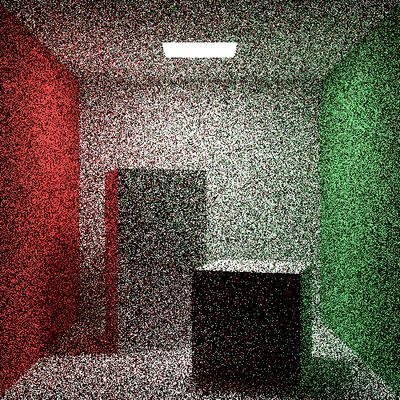
\includegraphics[width=\textwidth*\real{0.42}]{Images/noisy_image.jpeg}
	}
	\qquad
	\subfloat[Less noisy image]{
        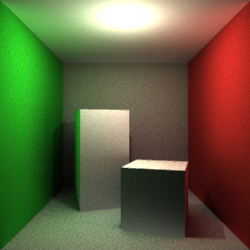
\includegraphics[width=\textwidth*\real{0.42}]{Images/less_noisy_image.png}
    }
	\caption{Noise in a ray traced image.}
    \label{fig:noise_example}
\end{figure}

Actually, in many ray tracing techniques, just one probe ray is cast, but the estimated light entering a point is temporally accumulated. This works because Monte-Carlo integration is unbiased.

\subsection{Variance Reduction Techniques}
In this section we will describe importance sampling, a variance reduction technique applicable to Monte-Carlo method to reduce the error of the estimate without increasing the number of samples. This technique is particularly relevant in ray tracing, since we have a very limited number of probe rays we can cast. Eventually, we will show how importance sampling can be applied to the ray tracing context, and how its usage generates artifacts in the ray distribution in the rendered scene.

Variance reduction techniques, as the name suggests, are methods used in the Monte-Carlo context to reduce the variance of the estimator without increasing the computational effort.

One of the variance reduction techniques employed in ray tracing and that is relevant to our work is called importance sampling (IS). Let's imagine that we want to integrate a constant function. In this case, the positions where we place our samples are irrelevant: each time we run the Monte-Carlo simulation, the estimator will return the same result, therefore the variance is always 0.

The intuitive idea of importance sampling is to try to run the Monte-Carlo simulation always on a constant function. From a theoretical point of view, this is extremely easy: we simply need to divide the integrand $\textit{f}$ by a function proportional to it. Given the general Monte-Carlo estimator, this can be achieved by choosing a sampling PDF $p$ proportional to $\textit{f}$:

$$\langle F^N \rangle = \frac{1}{N}\cdot\sum_{i=0}^{N-1}\frac{\textit{f}(X_i)}{p(X_i)} \longrightarrow \frac{1}{N}\cdot\sum_{i=0}^{N-1}\frac{\textit{f}(X_i)}{k\cdot \textit{f}(X_i)}$$

From an operative point of view, with importance sampling it is more likely to get a sample from a portion where the integrand has a high value, but, at the same time, this sample will have a lower weight in the final estimate (because it is divided by a higher value). Whereas, if we get a sample from a portion where the integrand has low values, which is rare, its weight will be bigger. This means that the estimate comes from a finer-grained sampling of the portions where the integrand carries most of its information.

Even though from a mathematical point of view this is simple, from a concrete standpoint the technique can be difficult to apply. The main reason is that in many cases, such as in ray tracing, we don't have an analytical form of the integrand function, therefore finding a function proportional to it is problematic. Moreover, a bad choice of the PDF, can lead to an increase in the variance of the estimator even compared to the uniform PDF.

Going back to the ray tracing context, the integrand function has this equation:

$$\int_\Omega BRDF(\bar{x}, \bar{\omega}_i, \bar{\omega}_o) \cdot \cos(\bar{n}, \bar{\omega}_i) \cdot L_i(\bar{x}, \bar{\omega}_i) d\bar{\omega}_i$$

It is possible to note that the function is made up of 3 terms: the $BRDF$, the geometry term and the incoming light term. We can therefore use a probability function proportional to one of the terms to reduce the variance:
\begin{description}
	\item[Cosine sampling] The sampling PDF is proportional to the geometry term of the rendering equation.
	\item[BRDF sampling] The sampling PDF is proportional to the BRDF. BRDFs can assume complex analytical forms, therefore sampling the BRDF is not always easy.
	\item[Light sampling] The sampling PDF should be proportional to the $L_i$ term of the rendering equation.
\end{description}

Light sampling is particularly problematic because we almost never have an analytical form of the $L_i$ function. The most used form of light sampling is called next event estimation (NEE), and is achieved by casting rays towards direct light sources. The way in which the light source to sample is chosen can be completely random or require complex strategies, such as in the case described in this article in the book \textit{Ray Tracing Gems}: \cite{multi_light_sampling}.

The main issue with next event estimation is that a direct light can be occluded by an object, or, conversely, a strong light could come from an indirect source, such as a reflection. For this reason, another technique, called path guiding \cite{path_guiding}, has been developed to consider mainly indirect lighting in the sampling PDF. Path guiding can be computationally expensive, therefore is often used in non-real-time scenarios, even though approximations have been proposed even for real-time ray tracing, such as \cite{real_time_path_guiding}.

\begin{figure}[H]
    \centering
    \subfloat[Next event estimation]{
        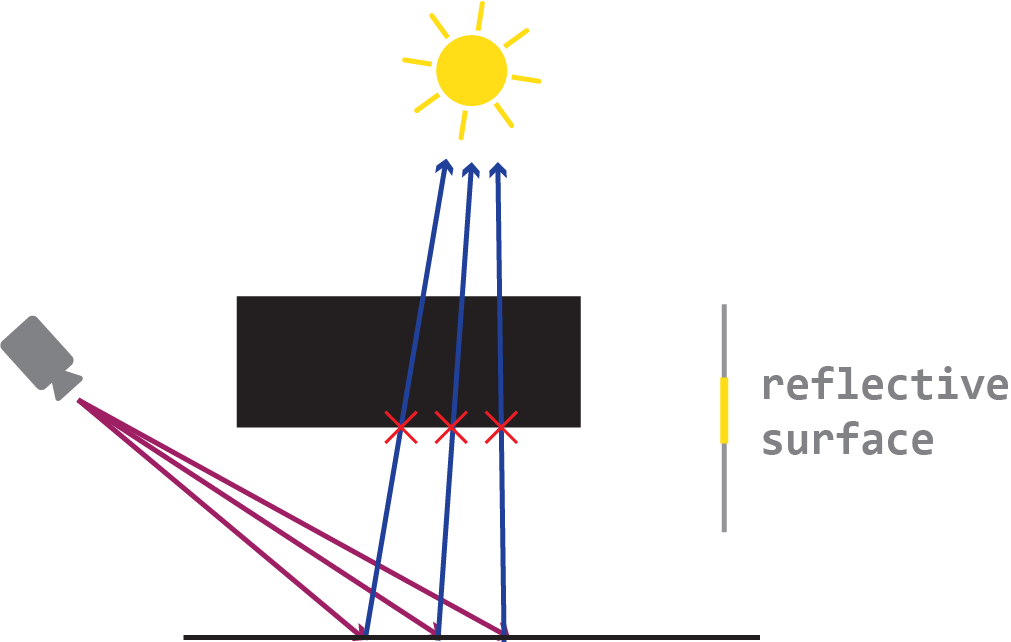
\includegraphics[width=\textwidth*\real{0.45}]{Images/nee.png}
	}
	\qquad
	\subfloat[Path guiding]{
        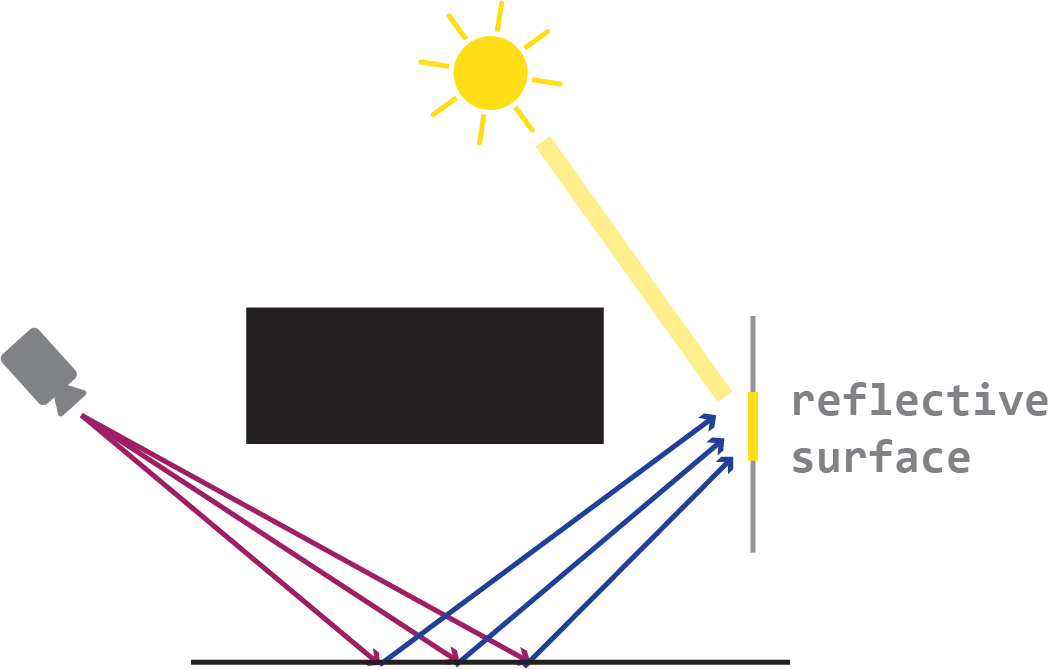
\includegraphics[width=\textwidth*\real{0.45}]{Images/path_guiding.png}
    }
	\caption{With NEE light is directly cast toward direct light sources. With path guiding, indirect illumination is taken into account in order to build a better sampling PDF, at a higher cost.}
    \label{fig:nee_and _path_guiding}
\end{figure}

Using BRDF sampling or light sampling in isolation as variance reduction PDFs can give better or worse results mainly based on the rendered section of the scene. For example, in a well illuminated scene with a mirror, using light sampling gives bad results. This happens because the BRDF of the mirror is null everywhere except for a spike in the perfect reflection direction. This means that its weight in the integrand is much more important than the weight of the $L_i$ term, which is almost constant being the scene well illuminated. If we use light sampling we will cast rays almost uniformly, and many of them will lose all of their energy as soon as they hit the mirror and reflect to a non-perfect-reflection direction.

On the contrary, in a scene with rough materials (such as concrete) and with few distant light sources, using light sampling would be beneficial, since many of the rays would be cast toward a light, instead of toward the void.

To remedy the problem of choosing the right importance sampling technique based on the portion of the scene, a new technique has been developed, called multiple importance sampling (MIS). Since the technique is an extension to importance sampling, it will be described in appendix \ref{ch:mis}.

The key take away from this section is that with importance sampling we use a non-uniform PDF to sample probe rays from. This creates artifacts in the ray distribution in the scene. In particular, if next event estimation is used, a big part of the rays will tend to go toward light sources. In chapter \ref{ch:projected_area_heuristic} we will study how these artifacts in the ray distribution can be exploited to design a faster technique to traverse a bounding volume hierarchy, which is the main subject of the next section \ref{sec:ray_tracing_acceleration_structures}.

\section{Ray Tracing Acceleration Structures} \label{sec:ray_tracing_acceleration_structures}
In this section we will describe the first family of software optimizations we talked about in section \ref{ssec:optimizations_overview}. These optimizations aim at reducing the time needed to find the intersections between a ray and the geometry of the scene. Usually this is achieved by organizing the scene geometry in a spatial data structure, or by wisely choosing the order in which rays are cast, in order to improve the spatial coherency of the data accesses on the GPU \cite{ray_coherency}. After a brief description of older acceleration structures, we will focus on the state-of-the-art acceleration data structure, called bounding volume hierarchy (BVH), and present how it is constructed. We will eventually show the assumptions on which the construction algorithm is based, whose refutation will be the main subject of the novel approach we propose in the next chapter \ref{ch:projected_area_heuristic}.

\subsection{The Need for Acceleration Structures}
As we've seen throughout this chapter, in any of the algorithms of the ray tracing family, casting rays is the core of the procedure. Rays are primarily cast from the camera toward the scene, and subsequently, based on the specific algorithm used, they hit objects and bounce off of them. Until now, however, we have overlooked how, in a concrete scenario, the algorithm can detect what is the object hit by the ray. 

Before delving into the algorithms that can be used to carry out this task, it is important to understand how an object is described in the world of computer graphics. In the history of computer graphics a lot of techniques to represent an object have been developed. Some examples are volumetric rendering with voxels \cite{voxel_rendering}, signed distance fields \cite{sdf} and implicit functions that work best with the ray marching algorithm \cite{ray_marching}, or point clouds. By the way, the most common method to represent 3D objects are polygonal meshes.

A polygonal mesh describes an object by defining its surface via points, edges and faces (usually triangles). Meshes's success derived from the fact that they were one of the first representations proposed in the world of computer graphics. This led to a big part of the research converging to this specific representation form. For example, GPUs are specialized for the rendering of trianglular meshes via rasterization, even though in the last few years their architecture has been made more flexible.

\begin{figure}[H]
    \centering
    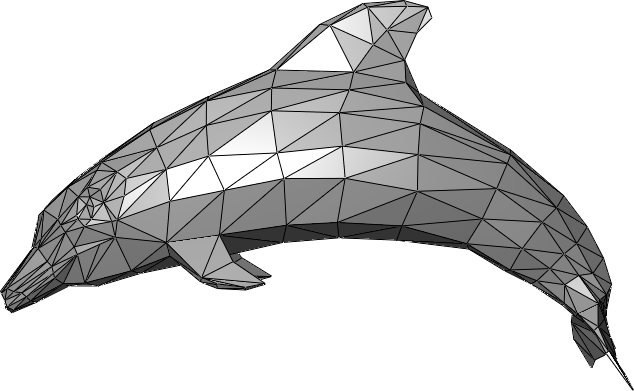
\includegraphics[width=\textwidth*\real{0.7}]{Images/triangular_mesh.png}
    \caption{A triangular mesh.}
    \label{fig:triangular_mesh}
\end{figure}

Meshes are also handy to create for graphic artists, and can be easily modeled to represent many kinds of objects, even though they are not suited to represent liquids or gases, such as clouds. Meshes, since they describe only the outside surface of an object, can prove difficult to use in applications where the interior is important, such as medical visualizations or games where objects can be dynamically destroyed. In these context it is usually preferred to employ voxels. Moreover meshes are a discrete representation, meaning that, once created, they cannot be used to visualize the details of the object at an arbitrary resolution, contrary to implicit functions. However, techniques to change the resolution based on the dynamic situation have been developed, such as LODing, tessellation \cite{tessellation} or more recent methods such as Nanite \cite{nanite}.

Regardless of their advantages and disadvantages, triangular meshes are by far the most used representation, therefore in this work we decided to focus on them in the scenario where the rendering technique is an algorithm of the ray tracing family.

In order to find the intersection between a ray and a list of meshes making up a scene, we need to test the intersections between the ray and all the triangles making up the meshes, and keep the closest one\footnote{In some scenarios, such as when we just want to check for occlusion, it is not necessary to find the closest intersection, but just to find an intersection. In this case some optimizations can be developed, but the core concepts remain the same.}.

The naive way of detecting the intersection is the brute-force solution to iterate over all of the triangles and storing the closest intersection found so far. The algorithm we used to detect the intersection between a ray and a triangle in our implementation can be found in appendix \ref{sec:ray_triangle_intersection}. Despite working, this method cannot be practically used either in real-time scenarios, nor in non-real-time ones. The problem resides in the fact that there are too many triangles to test against. Even in a non-real-time case this approach would be too expensive, because, even if the time budget for a frame is big, meshes created for non-real-time purposes usually have a way higher triangle resolution, and also way more rays to trace. From a complexity point of view, tracing a scene with $n$ triangles and $m$ rays in this way has complexity $\mathcal{O}(m\cdot n)$.

This is the reason why acceleration structures have been developed. Most of the acceleration structures organize the triangles in a hierarchical fashion, so that it is possible to exclude a big chunk of them if a ray doesn't hit certain parts of the scene. One very simple example of acceleration structure would be to divide the scene into 2 parts and keep track of what triangles reside on each one. Now, if a ray doesn't hit one of the 2 parts, it is possible to exclude all of the triangles contained in that region, without having to test them one by one.

Acceleration structures can be divided into 2 categories:
\begin{description}
	\item[Space partitioning] The space is recursively subdivided into disjoint regions. Objects (triangles) can potentially appear in more than one region, if they are overlapping. 
	\item[Object partitioning] Objects are subdivided into disjoint sets, enclosed into spatial regions. The regions can potentially be overlapping.  
\end{description}

Historically, initially the first family of acceleration structures has been used, but todays state-of-the-art acceleration structure is the BVH, part of the second family. We will now very briefly list some of the most famous acceleration structures historically used for ray tracing, and, in the next section, we'll diffusely talk about the BVH.

The first space partitioning acceleration structure developed is the uniform grid. In this structure the 3-dimensional space of the scene is subdivided into static fixed-sized cells in a regular pattern. Then, each triangle is assigned to all the cells it at least partially covers. This can be at least a single cell, to, potentially all the cells of the scene. When a ray is traced, first, a cell it intersects is found, and then, all the triangles inside this cell are tested against the ray. This is repeated for all the cells the ray hits in its path. If an intersection $P$ is found, then, all the cells that are at a further distance from the ray origin than $P$ can be discarded without testing individual triangles.

\begin{figure}[H]
    \centering
    
\includegraphics[width=\textwidth*\real{0.5}]{Images/TODO.png}
    \caption{The uniform grid in 2D.}
    \label{fig:uniform_grid}
\end{figure}

The uniform grid, while being an improvement over the brute-force approach, still lacks adaptability. Based on how the scene is composed, it is possible for some cells to be empty and others overcrowded. Moreover, as in any space partitioning data structure, it is possible that a triangle is tested more than once if it overlaps more than one cell. This could be avoided by using some intersection caching techniques, such as mailboxing \cite{mailboxing}.

In order to solve the adaptability problem of the uniform grid, octrees started being used. An octree is another 3D spatial data structure, and it is a tree where each node has 8 children. To subdivide a node into 8 children, it is divided by 3 planes, one perpendicular to each dimension, passing from the center of the parent node. This process is recursively executed until a specified amount of objects (triangles) remains inside a single node, or until the depth of the tree gets past a threshold. Since the octree is a complete tree, and the size and center of each child can be automatically computed starting from the size of the root and the level\footnote{$size_{children} = size_{root} / 2^{level}$ given that the root has level $0$.}, it is possible to store the octree in an implicit array structure, making it more efficient both from an access pattern and space point of view.

\begin{figure}[H]
    \centering
    
\includegraphics[width=\textwidth*\real{0.5}]{Images/TODO.png}
    \caption{A 2D octree..}
    \label{fig:octree}
\end{figure}

It is important to note how octrees adapt better to the scene. Indeed, compared to fixed grids, they alleviate the \textit{teapot in the stadium} problem, namely the issue that appears when there is a scene with different densities of objects. For example, precisely what happens when we have a small but high-resolution object (a teapot), inside a big and mostly empty space (a stadium). With octrees this problem is handled by having few big and empty cells in the regions where there is a low density of triangles, and many small cells where there are high-resolution objects. In this way less memory is wasted, and even traversal is improved. Indeed, if a ray passes through empty space, just few cells must be checked, instead of a bigger amount as in the case of a uniform structure like the fixed grid. Conversely, in case a ray goes through a dense region, fewer triangle tests will be carried out, because the cells the ray intersects are smaller and not overcrowded. Another advantage of octrees is that they are a tree data structure. This implies that if a node is not hit by a ray, all its children can be immediately discarded.

\begin{figure}[H]
    \centering
    
\includegraphics[width=\textwidth*\real{0.5}]{Images/TODO.png}
    \caption{How an octree adapts to a \textit{teapot in the stadium} kind of scene.}
    \label{fig:octree_teapot_stadium}
\end{figure}

Another structure that is a generalization of octrees and delivers similar performance is the kd-tree. In 3D kd-trees each node is split into 2 children by a plane. At each level the plane is perpendicular to one of the dimensions, in a round-robin fashion (for example, at level 0 it is normal to $x$, at level 1 to $y$, at level 2 to $z$ and so on). Differently from octrees, the plane doesn't necessarily have to pass through the center of the parent node, making their construction even more flexible.

\begin{figure}[H]
    \centering
    
\includegraphics[width=\textwidth*\real{0.5}]{Images/TODO.png}
    \caption{A kd-tree in 2D.}
    \label{fig:kd_tree}
\end{figure}

These are the most prominent spatial data structures used for ray tracing. However, nowadays an object partition structure is used, called bounding volume hierarchy, which we will analyze in the next section.

\subsection{The Bounding Volume Hierarchy}
A BVH \cite{bvh_primer} is a binary tree\footnote{Technically it can be a tree with any breadth, but binary trees are the most common ones.} where each node wraps some of the triangles in the scene in a bounding volume. Given a node $A$ wrapping the triangles in the set $T_A$, then the two children of $A$, called $B$ and $C$, wrap the triangles in the sets $T_B$ and $T_C$ such that $T_B \cup T_C = T_A$. Thanks to this structure, if a ray doesn't intersect a bounding volume, we deduce that it will not intersect any of the triangles contained in the bounding volume too, making it possible to discard them without having to perform any additional intersection test.

Assuming the best-case scenario where a ray always hits only one of the 2 children of a given node during traversal, if the BVH is balanced and has one triangle per leaf, then the complexity of finding an intersection between a ray and the scene is $\mathcal{O}(log_2(n))$, where $n$ is the number of triangles. This is not always the case, since it often happens that a ray hits both the children of a given node. One of the heuristics that we propose in this thesis in chapter \ref{ch:splitting_plane_facing_technique}, aims at reducing the number of this expensive situation, by building the BVH in a smart way.

The bounding volume in which a BVH encloses triangles should have a form that is cheap to intersect with a ray, and also cheap to build given a set of triangles.

A choice can be a sphere, which is easy to test against a ray. Moreover, building the tightest enclosing sphere given a set of triangles is as simple as finding the 2 triangles furthest away in each direction, computing the middle point and setting as radius the distance between the furthest triangle and the middle point. The negative aspect of using bounding spheres lies in the fact that a sphere extends equally in all directions in 3D space. This means that if the triangles are displaced in a way where they extend more in one direction than in other ones, the bounding sphere will present a lot of slack space, and won't enclose the triangles thightly. This is not ideal, because in the traversal phase a non-tight bounding volume generates a lot of false positives, namely situations where the bounding volume is hit but no triangle is intersected.

\begin{figure}[H]
    \centering
    
\includegraphics[width=\textwidth*\real{0.4}]{Images/TODO.png}
    \caption{Bounding circle (2D bounding sphere) can present large slack spaces.}
    \label{fig:bounding_sphere}
\end{figure}

At the opposite side of the spectrum there are polygonal bounding volumes. In this case they are able to thightly enclose the triangles, but building them is not easy, and intersecting them can prove as expensive as intersecting the set of triangles itself.

Another option is using oriented bounding boxes (OBB). Oriented bounding boxes in 3D are rectangle parallelepiped. This means that they can have a different extension in 3 different arbitrary directions (each one perpendicular to the remaining two), making them better at tightly enclosing any distribution of triangles compared to spheres. However, computing a tightly enclosing OBB starting from the set of triangles involves using the principal component analysis \cite{obb_construction}, which can be too expensive in real-time scenarios. Moreover, intersecting a ray against an OBB involves a rotation transformation, which, again, can be too slow, especially during the traversal phase. In general OBBs are too slow in many scenarios, but, given their ability to tightly enclose triangles, can be used along with AABBs \cite{obbs_for_bvhs}.

\begin{figure}[H]
    \centering
    
\includegraphics[width=\textwidth*\real{0.4}]{Images/TODO.png}
    \caption{A 2D OBB.}
    \label{fig:obb}
\end{figure}

Axis-aligned bounding boxes (AABB) are the most used bounding volumes. AABBs are OBBs that have no rotation, and are always aligned with the cartesian axes. This means that AABBs can indeed have a different extension in 3 directions, but the directions are limited to the ones of the cartesian axes. These limitations make them worse at tightly enclosing triangles than OBBs, but at the same time make it way easier to build them and intersect them with a ray. To build an AABB starting from a set of triangles, it suffices to iterate over all the triangles and keep track of the minimum and maximum point in all 3 dimensions. An AABB is then fully described by its minimum and maximum point. The algorithm to test whether a ray intersects an AABB is fast and can be implemented in a GPU-friendly branchless way, as described in appendix \ref{sec:ray_box_intersection}.

\begin{figure}[H]
    \centering
    
\includegraphics[width=\textwidth*\real{0.4}]{Images/TODO.png}
    \caption{A 2D AABB.}
    \label{fig:aabb}
\end{figure}

AABBs are the most used bounding volumes both in real-time and non-real-time ray tracing. For this reason, from now on, when we refer to a BVH we will always consider the case of a BVH based on AABBs.

\begin{figure}[H]
    \centering
    
\includegraphics[scale=0.4]{Images/TODO.png}
    \caption{A 2-dimensional BVH.}
    \label{fig:bvh_2d}
\end{figure}

Despite it is not clear that BVHs' raw performance is better than kd-trees', especially on large scenes \cite{bvh_vs_kd_tree}, they became the state-of-the-art acceleration structure for many practical reasons.

First of all, being an object partitioning data structure, they can solve the \textit{teapot in a stadium} problem even better than kd-trees. This is because it is possible to completely cut off empty space, as it is possible to observe in figure \ref{fig:bvh_2d}.

Moreover, and this is especially relevant in a dynamic real-time scenario such as a videogame, BVHs are easier to update when the geometry of the scene changes \cite{bvh_update}.

BVHs construction algorithm is also simpler than kd-trees', allowing a faster build-time, which can be crucial in highly dynamic real-time applications. And they also have a smaller memory footprint compared to kd-trees, as mentioned in \cite{bvh_spatial_splitting} and \cite{bvh_advantages}.

\subsection{BVH Construction}
Building the optimal BVH according to some metric is an NP-complete problem. In order to do so the algorithm would have to build all the possible BVHs given a set of triangles, compute the metric and keep the best one. The number of possible different binary trees grows factorially with the number of leaves. Given $n$ leaves, the number of possible binary trees is the $n-1$ Catalan number \cite{catalan_numbers}: $C_{n} = \frac{(2n)!}{(n+1)! \cdot n!}$. The number of possible BVHs is even bigger, because, since a leaf can contain more than one triangle, it is not a given that the number of leaves corresponds to the number of triangles.

Given that building the optimal BVH is not feasible even in a non-real-time scenario, research started studying methods to build a BVH with an acceptable quality faster. This resulted in the use of greedy algorithms and heuristics.

The base algorithm fo building a BVH can be summarized in these steps:
\begin{algorithm}[H]
	\caption{Summarized BVH construction algorithm.}
	\begin{algorithmic}[1]
		\Function{BuildBvh}{$triangles$}
		\Let{$leftNode$}{[\;]}
		\Let{$rightNode$}{[\;]}
		\Let{$cost$}{$\infty$}
		\Loop{$\;cost < threshold \AOr all\;possible\;splits\;tried$}
			\Let{$[leftNodeTmp, rightNodeTmp]$}{$SplitTriangles(triangles, howToSplit)$}
			\Let{$costTmp$}{$ComputeCost(leftNodeTmp, rightNodeTmp)$}
			\If{$costTmp < cost$}
				\Let{$leftNode$}{$leftNodeTmp$}
				\Let{$rightNode$}{$rightNodeTmp$}
				\Let{$cost$}{$costTmp$}
			\EndIf
		\EndLoop
		\If{$\ANot StopCriterion(cost, leftNode, rightNode)$}
			\State{$BuildBvh(leftNode.triangles)$}
			\State{$BuildBvh(rightNode.triangles)$}
		\EndIf
		\EndFunction
	\end{algorithmic}
	\label{alg:bvh_construction_summary}
\end{algorithm} 

The proposed algorithm is a greedy one. This means that it tries to minimize the cost function locally, at each level of the BVH, but when a decision is taken, it is not possible to change it. Making the local optimal choice doesn't imply that the global minimum of the cost function will be found, but at least it makes the problem tractable.

The algorithm can be divided into 3 steps: triangles splitting, cost computation and stopping criterion.

\subsubsection*{Stopping Criterion}
The stopping criterion phase decides whether the $BuildBvh$ function should make the recursive call and split the new children nodes. The stopping criterion can be based on different metrics, among which:
\begin{itemize}
	\item Children cost
	\item Total triangles in children
	\item BVH level
\end{itemize}

\subsubsection*{Triangles Splitting}
Given the set of triangles of the parent node, in this phase the algorithm tries to split them into two subsets and build the enclosing bounding volumes.

In order to split the triangles into two subsets, a plane is chosen, and based on which side of the plane the barycenter of each triangle is, the triangle is assigned to one of the two subsets. This means that it is possible that a triangle has some vertices in the opposite semispace compared to the one it has been assigned to. This is one of the reasons why two children can have some of their volumes overlapping. 

\begin{figure}[H]
    \centering
    
\includegraphics[scale=0.4]{Images/TODO.png}
    \caption{Triangles splitting via arbitrary plane.}
    \label{fig:triangles_splitting}
\end{figure}

As shown by \cite{bvh_overlapping_metric} too much overlapping between children nodes leads to a decrease in the quality of the final BVH. For this reason, in chapter \ref{ch:splitting_plane_facing_technique} we propose a novel technique trying to take into account the overlapping during this phase of BVH construction.

In order to choose which plane to use to split the triangles, some optimizations can be employed. In BVHs based on AABBs it is useful to try to split the triangles only in the 3 cartesian directions. Usually just one of the directions is chosen, in order to further optimize the process. The way in which the direction is chosen can vary based on the methods used. An often employed technique is to cut along the longest dimension of the parent AABB. Another one is to cut in a round-robin fashion, similar to what is done in kd-trees. In chapter \ref{ch:splitting_plane_facing_technique} we propose a novel method, as mentioned above.

Another advantage of using only the 3 cartesian directions is that in order to detect the semispace a point falls into, it is sufficient to compare one of its coordinates with the coordinates of a point the plane is passing through. This is an optimization compared to computing the cross-product like in the case where the plane has an arbitrary normal direction.

After choosing a splitting direction, all possible cuts in that direction should be tested. Given an amount on $n$ triangles to be splitted, trying all the possible cuts in one direction means trying $n-1$ subdivisions, where the splitting plane is placed each time on the barycenter of a triangle. Since $n$ can be a big number, especially while running the algorithm on the first levels of the BVH where nodes are big, a technique called binning can be introduced.

With binning, instead of trying every possible cut, a predefined number of cuts is attempted. The splitting plane is translated each time by a fixed length (a bin) along the chosen cutting direction from the position of the previous cut. By using binning it is possible to miss some of the possible cuts, especially in a region dense of triangles. However, the most relevant cuts are often positioned where there is a big gap in one direction between two consecutive triangles. This is because it is possible to leverage the big gap to cut off as much space as possible. Whereas, if the gap is small, it is likely that the resulting children nodes' AABBs overlap. For this reason binning is an efficient approximation, especially in the higher levels of the BVH.

\begin{figure}[H]
    \centering
    \subfloat[Triangles splitting without binning]{
        
\includegraphics[width=\textwidth*\real{0.42}]{Images/TODO.png}
	}
	\qquad
	\subfloat[Triangles splitting with binning]{
        
\includegraphics[width=\textwidth*\real{0.42}]{Images/TODO.png}
    }
	\caption{With binnin it is possible to lose some cuts, but the most relevant ones are always found.}
    \label{fig:triangles_splitting_binning}
\end{figure}

After generating the two subsets of triangle, the enclosing AABBs must be built. The process to build an AABB from a set of triangles is straight-forward, and is summarized by this algorithm:
\begin{algorithm}[H]
	\caption{AABB building from triangles set.}
	\begin{algorithmic}[1]
		\Function{BuildAabb}{$triangles$}
		\Let{$min$}{$(\infty,\infty,\infty)$}
		\Let{$max$}{$(-\infty,-\infty,-\infty)$}
		\ForAll{$t \in triangles$}
			\Comment{$t.v_k$ is the $k^{th}$ vertex of the triangle $t$}
			\Let{$min.x$}{$Min(min.x, t.v_0.x, t.v_1, t.v_2.x)$}
			\Let{$max.x$}{$Max(max.x, t.v_0.x, t.v_1, t.v_2.x)$}
			\Let{$min.y$}{$Min(min.y, t.v_0.y, t.v_1, t.v_2.y)$}
			\Let{$max.y$}{$Max(max.y, t.v_0.y, t.v_1, t.v_2.y)$}
			\Let{$min.z$}{$Min(min.z, t.v_0.z, t.v_1, t.v_2.z)$}
			\Let{$max.z$}{$Max(max.z, t.v_0.z, t.v_1, t.v_2.z)$}
		\EndFor
		\State \Return $Aabb(min, max)$
		\EndFunction
	\end{algorithmic}
	\label{alg:aabb_creation}
\end{algorithm} 

\subsubsection{Cost Computation - Surface Area Heuristic} \label{ssec:cost_computation}
In the previous section we have described how a standard BVH construction algorithm can split the triangles of a node into two subsets, and compute the AABB for each one of them. In this section we will analyze how the algorithm decides whether a split is better than another one.

To choose the best split, a BVH construction algorithm sorts the splits proposed by the splitting triangles phase by assigning to each one a value through a cost function. 

The aim of a cost function is to accurately predict how \textit{good} the final BVH will be. The concept of \textit{goodness} or \textit{quality} of a BVH is directly related to how fast an arbitrary ray is able to traverse it to find the first intersection with a triangle. It is possible to evaluate the cost function for every node as if it was a leaf node, and this is useful while building the BVH with the greedy algorithm. It is also possible to compute the cost function of the overall BVH, which is used to evaluate the quality of the BVH built.

The most used cost function is called surface area heuristic (SAH), and is based on a very simple idea: the smaller the surface area of a node's AABB, the less likely is for this node to be hit by a ray. If a node is hit less times by a ray, it means that fewer checks are needed to traverse the BVH, therefore its quality, as we defined it above, is higher.

Given an AABB, it is trivial to compute its surface area as: 
$$A=(max_x-min_x)\cdot (max_y-min_y) + (max_x-min_x)\cdot (max_z-min_z) + (max_y-min_y)\cdot (max_z-min_z)$$

Now, we would like to have a cost function that is agnostic to the absolute size of the scene. For this reason, instead of using directly the surface area to compute the cost metric, we transform it into the probability that a ray hits a specific node.

To do so SAH makes some reasonable assumptions on some properties of the rays in the scene:
\begin{itemize}
	\item A ray always hits the AABB enclosing the whole scene;
	\item All rays have origin outside the AABB enclosing the whole scene, and their positions are uniformly distributed;
	\item Rays never intersect any primitive, and are infinitely long;
	\item Rays are uniformly distributed in their direction space.
\end{itemize}

With these assumptions in place, which we'll analyze better in section \ref{sec:sah_hypotheses_fall}, we can define the probability a ray hits a node $K$ as:
$$p(ray\; hits\; K) = \frac{Area_K}{Area_{root}}$$

Since all rays hit the root AABB, we can interpret it as the certain event. And since the rays' directions are uniformly distributed, the surface area can be mathematically interpreted as a measure of how likely it is for a ray to hit an AABB.

\begin{figure}[H]
    \centering
    
\includegraphics[scale=0.5]{Images/TODO.png}
    \caption{Visual relationship between AABB area and hit probability in 2D, under the assumption rays are uniformly distributed.}
    \label{fig:area_probability_visual}
\end{figure}

Finally, in order to compute the cost function, we have to also take into account the cost of the intersection test between a ray and a triangle, and a ray and an AABB. In literature a cost of $1.2$ is assigned to the first test, and a cost of $1$ to the second one.

We now have all the elements to define the SAH cost function for a node $K$:
$$Cost_{SAH}(K) = \frac{Area_K}{Area_{root}} \cdot \#triangles_K \cdot 1.2$$

The $\#triangles_K \cdot 1.2$ part tells us that when this node is hit by a ray, a ray-intersection test per triangle must be carried out. The term $\frac{Area_K}{Area_{root}}$ weights the cost of computing the ray-intersection tests with the probability that this node is actually hit. This means that, even if a node has a lot of triangles in it, if these triangles are all packed in a small region, the cost of the node will not be too high, because it is unlikely for a ray to hit the node in the first place.

It is important to note that this formula returns the cost of a node in isolation. But the nodes we are dealing with are part of a BVH. In other words, when an internal node of a BVH is hit, this doesn't trigger a ray-triangle test for all of its triangles (as suggested by the formula), but only recursively triggers ray-AABB tests against its two children. Only when this formula is used on leaf nodes, the returned cost actually reflects the real cost of a ray intersecting the node.

Therefore why are we suggesting to use this formula? The answer is that we are building the BVH with a greedy algorithm. When we have to evaluate a node, we have no way of knowing how its children will be, therefore the only way is to estimate its cost as if it didn't have any children at all, as if it was a leaf node.

However it is also useful to have a way to evaluate the cost of a BVH a-posteriori. In this case, based on the node type, we can have two situations:
\begin{description}
	\item[Leaf node] The cost of a leaf node can be computed with the same formula we have analyzed, for the reasons we have stated above.
	\item[Internal node] When an internal node is hit, the next step of the traversal is to perform a ray-AABB test with each one of the two children. Therefore the cost is: $Cost_{SAH}(K_{intern}) = \frac{Area_K}{Area_{root}} \cdot 2 \cdot 1$. 
\end{description}

By merging the formulae to compute the cost of leaf and internal nodes, the cost function of a BVH assumes this form:
$$Cost_{SAH}(BVH) = \sum_{L \in leaf\; nodes} \frac{Area_L}{Area_{root}} \cdot \#triangles_L \cdot 1.2 + \sum_{I \in internal\; nodes} \frac{Area_I}{Area_{root}} \cdot 2 \cdot 1$$

\chapter{Projected Area Heuristic} \label{ch:projected_area_heuristic}
In chapter \ref{ch:background_theory} we have described how ray tracing works. In particular, in section \ref{sec:monte_carlo_and_variance_reduction_techniques} we have seen how importance sampling generates artifacts in the ray distribution of the scene. In section \ref{sec:ray_tracing_acceleration_structures} we described how it is possible to build an acceleration structure to speed up the ray-scene intersection process, and we have shown how the surface area heuristic is the state-of-the-art method to build high-quality BVHs. In this chapter, we will show that some of the hypotheses of the SAH are not satisfied in a real-world scenario, due to the use of importance sampling. We will eventually propose a new heuristic called projected area heuristic (PAH), and show the situations where it can be used to build BVHs. In this chapter we will describe the problem and the solutions from a theoretical point of view; all the implementation details will be thoroughly discussed in section \ref{TODO}.

\section{SAH Hypotheses Fall} \label{sec:sah_hypotheses_fall}
In section \ref{sec:ray_tracing_acceleration_structures} we have seen that the surface area heuristic, used to build high-quality BVHs with the described greedy algorithm, works under these hypotheses:
\begin{itemize}
	\item A ray always hits the AABB enclosing the whole scene;
	\item All rays have origin outside the AABB enclosing the whole scene, and their positions are uniformly distributed;
	\item Rays never intersect any primitive, and are infinitely long;
	\item Rays are uniformly distributed in their direction space.
\end{itemize}

In a standard situation, the first hypothesis can be considered true for all the rays. It is still possible, in some scenarios, that a part of the rays doesn't hit the scene. Examples can be found in the discussion on the test cases for our thesis in chapter \ref{TODO}, however, in most scenarios all the rays hit the scene, because casting a ray away from the scene would be wasteful.

For what concerns the second hypothesis, the situation is completely different. Indeed, in many applications the camera is inside the scene, therefore the rays' origin is inside the scene too. But even in a situation where the camera is placed outside the scene, still the majority of rays would have origin inside. This happens because in many algorithms of the ray tracing family, the primary rays (rays cast from the camera position) are in a much smaller number than the secondary rays. With secondary rays we refer to what we called in the previous chapter \textit{probe rays}, namely those rays originating after a ray-triangle intersection. As we have seen, generating probe rays to evaluate the rendering equation is a recursive process, and in order to obtain an image with an acceptable amount of noise, a lot of probe rays must be cast.

Studies about this issue with the surface area heuristic have been carried out. For example, in this article \cite{sah_interior_rays}, Fabianowski et al. divide the scene into discrete regions, and try to evaluate the hit probabilities from the center of each one.

The third and fourth hypotheses have both to do with how the rays are distributed in the 3D space of the scene. It is easy to see how the third hypothesis doesn't hold true in a real-world scenario. Of course primitives will block rays, thus potentially creating regions of the scene where few or no rays are present (imagine the region of space inside an opaque box, or even more in general, the space inside the boundaries of meshes). 

For what concerns the last hypothesis, we have to remember how Monte-Carlo integration works. In theory, after a ray hits an object, there is an equal probability it bounces toward any direction in the hemisphere. This behavior, considering that the other hypotheses hold true, would create a uniform distribution of rays in the scene. However, as we have seen in section \ref{sec:monte_carlo_and_variance_reduction_techniques}, importance sampling makes it so that the probe rays distribution is not uniform. In particular, if direct light sampling is used, a lot of probe rays will tend to go toward light sources. This artifact in the ray distribution shows how not even the last SAH hypothesis holds true.

\begin{figure}[H]
    \centering
	\subfloat[Without importance sampling]{
    	
\includegraphics[width=\textwidth*\real{0.45}]{Images/TODO.png}
	}
	\qquad
	\subfloat[With importance sampling]{
    	
\includegraphics[width=\textwidth*\real{0.45}]{Images/TODO.png}
	}
    \caption{With importance sampling rays are not distributed uniformly in the scene.}
    \label{fig:non_uniform_rays}
\end{figure}

Since rays are not distributed uniformly in the scene, it means that we cannot interpret the surface area of the AABB as related to the probability a ray hits it (figure \ref{fig:area_probability_visual}). For example, if an almost flat, but long AABB is present in a region where rays are parallel to the longest side of the AABB, the probability one of the ray hits it is very low. This wouldn't be reflected by the surface area of the AABB, which would assume a big value because of its long side. This can be visualized in the image below (\ref{fig:flat_long_aabb}).

\begin{figure}[H]
    \centering
    
\includegraphics[width=\textwidth*\real{0.5}]{Images/TODO.png}
    \caption{A flat but long AABB in a region of rays parallel to its long side.}
    \label{fig:flat_long_aabb}
\end{figure}

The first novel contribution of this work is based exactly on this simple observation, and on the refutation of the last hypothesis of surface area heuristic. In the next sections we will describe two relevant ray distributions that organically form in the scenes, due to the use of direct light importance sampling.

In the past other works on this same topic have been written, but the proposed solution was based on a very different approach. For example, in this paper \cite{distribution_aware_bvhs} Yan Gu et al. proposed to modify an already existing BVH based on some statistics harvested during the previous frames. In summary, if a node is rarely hit, its subtree is collapsed, and all the triangles in the subtree are directly placed in the node, which becomes a leaf. Conversely, frequently hit leaves become internal nodes, and are further divided.

In our approach, instead, we try to directly build a BVH aware of the ray distribution. To achieve this we propose a new heuristic to calculate the probability that a node is hit by a ray: the projected area heuristic (PAH).

\section{Parallel Ray Distribution} \label{sec:parallel_ray_distribution}
One of the relevant ray distributions that can naturally arise in a ray traced scene where light importance sampling is used, is the distribution where rays are all parallel among themselves. This ray distribution usually arises in proximity of plane area light sources.

\begin{figure}[H]
    \centering
    
\includegraphics[width=\textwidth*\real{0.5}]{Images/TODO.png}
    \caption{Parallel rays distributions arise in proximity of plane area light sources.}
    \label{fig:parallel_rays_distribution}
\end{figure}

In a 3-dimensional region with such a ray distribution, we can estimate the probability an AABB is hit by a ray by computing the area projected by the AABB on the plane having a normal vector parallel to the rays.

Let us first analyze the case where the rays are parallel to one of the 3 cartesian axis, let's say $z$. In this case, the extension of an AABB in the $z$ direction is irrelevant, because it is impossible for a ray to hit the box on any face other than the $xy$ ones. Therefore, only the area of the $xy$ face is related to the probability that the AABB is hit.

\begin{figure}[H]
    \centering
    
\includegraphics[width=\textwidth*\real{0.5}]{Images/TODO.png}
    \caption{If rays are parallel to a cartesian axis, the extension of the AABB in that dimension is irrelevant.}
    \label{fig:rays_parallel_to_cartesian_dimension}
\end{figure}

We can generalize this idea to the case where the rays are parallel to an arbitrary direction by orthographically projecting the AABB on the plane normal to the rays. The area of the orthographic projection is directly related to the probability a ray hits the AABB.

\begin{figure}[H]
    \centering
    
\includegraphics[width=\textwidth*\real{0.5}]{Images/TODO.png}
    \caption{Orthographic projection of an AABB.}
    \label{fig:aabb_ortho_projection}
\end{figure}

The details of our implementation will be extensively discussed in section \ref{TODO}.

\section{Point Ray Distribution} \label{sec:point_ray_distribution}
Another ray distribution commonly found in proximity of point lights is what we call the point ray distribution. In this distribution, rays all pass through the same point in 3D space, creating a radial pattern over a solid angle, as it is shown in the figure below.

\begin{figure}[H]
    \centering
    
\includegraphics[width=\textwidth*\real{0.5}]{Images/TODO.png}
    \caption{Point rays distributions arise in proximity of point light sources.}
    \label{fig:point_rays_distribution}
\end{figure}

Also in this case we can observe a relationship between the probability an AABB in this area is hit by a ray, and the area of the projection of said AABB. However, this time, the projection to estimate the hit probability is the perspective projection. The point all the rays in this region pass through can be interpreted as the focal point of the perspective. The projection plane can be placed at any distance from the focal point. Indeed, while it is true that by placing the plane at different positions we would get projections of different absolute sizes, it is also true that what we are really interested in is the relative area among the AABBs projected on the same plane. Indeed, as it is possible to see from the formula in section \ref{ssec:cost_computation} that we will report here:
$$p(ray\; hits\; K) = \frac{Area_K}{Area_{root}}$$
The hit probability $p$ is computed as the ratio between two areas.

\begin{figure}[H]
    \centering
    
\includegraphics[width=\textwidth*\real{0.5}]{Images/TODO.png}
    \caption{Perspective projection of an AABB.}
    \label{fig:aabb_perspective_projection}
\end{figure}

\section{The Projected Area Heuristic} \label{sec:projected_area_heuristic}
In the last two sections (\ref{sec:parallel_ray_distribution} and \ref{sec:point_ray_distribution}) we have seen how computing the projected area where there are certain ray distributions can be a better estimate for the probability that a ray hits an AABB, compared to the surface area. In simple words, this happens because some parts of the AABB are less likely (if at all) to be hit by a ray depending on their orientation compared to the rays present in that 3D region. 

With this notion, it is now easy to define a heuristic to be used during BVH construction and another one for BVH evaluation. Indeed we can use the exact same formulae used for the surface area heuristic, but with the projected area in place of the surface area of the AABBs:
$$Cost_{PAH}(K) = \frac{ProjArea_K}{ProjArea_{root}} \cdot \#triangles_K \cdot 1.2$$
$$Cost_{PAH}(BVH) = \sum_{L \in leaf\; nodes} \frac{ProjArea_L}{ProjArea_{root}} \cdot \#triangles_L \cdot 1.2 + \sum_{I \in internal\; nodes} \frac{ProjArea_I}{ProjArea_{root}} \cdot 2 \cdot 1$$

With this heuristic it is possible to build a BVH for a portion of the scene where there is a certain ray distribution. If there is a parallel ray distribution, the orthographic projected area will be used. Instead, if there is a point ray distribution, perspective projection should be used.

However, in a scene, there likely is more than a single and global ray distribution. It is possible that ray distributions are localized in definite regions of the scene. This means that, rather than building a single and global BVH valid for all the scene, it is necessary to build partial and localized BVHs for specific regions. This is the main topic of the next chapter \ref{ch:multi_influence_areas}.


\chapter{Multiple Influence Areas and the Top Level Structure} \label{ch:multi_influence_areas}
In this chapter we will show how it is possible to deal with a scene where there are multiple localized ray distributions. We will first introduce the problem in detail and with visual examples, then we will define the concept of ray affinity to region where a relevant ray distribution is present. Eventually we will show how a scene with multiple ray distributions can be traversed by a ray. In this chapter we won't explain all the implementation details of the solution we propose, that will instead be discussed in section \ref{TODO}.

As we have touched on in the last chapter, while ray tracing a scene, it is likely that more than a single relevant ray distribution appears. It is even more likely that, even if only one relevant distribution is present, it doesn't cover the entirety of the scene. For cases like these, it is necessary to be able to recognize whether a ray is affine to a certain ray distribution present in a scene. In case the ray is affine, we can use the BVH built with PAH on that part of the scene to find the first intersection. In case it is not affine, we must fall back to a global BVH, covering the whole scene. The definition of the term \textit{affine} is given in the next few paragraphs.

\begin{figure}[]
    \centering
    
\includegraphics[width=\textwidth*\real{0.7}]{Images/TODO.png}
    \caption{A scene with multiple relevant ray distributions.}
    \label{fig:multiple_ray_distributions}
\end{figure}

From this point on, we will refer to a 3D region of a scene where a relevant ray distribution is present as influence area. If the ray distribution is parallel (section \ref{sec:parallel_ray_distribution}), we call the region plane influence area. If the ray distribution is radial (section \ref{sec:point_ray_distribution}), the influence area is qualified as point influence area. Each influence area has an associated BVH (also called local BVH) built with PAH, where the projection method (orthographic or perspective) is the corresponding one to the ray distribution of the influence area.

Influence areas must first be localized in the scene. To do so, we decided to encode a plane influence area as an oriented bounding box. The rays start from one of the faces of the OBB, and are perpendicular to it. For what concerns point influence areas, the most natural bounding volume to localize them is 3D is a frustum. Rays start from the near plane of the frustum, and go toward the far plane. The direction of any of the ray can be obtained by connecting the origin of the ray on the near plane to the focal point of the frustum. In section \ref{TODO} it will be explained how we encoded the influence areas in our implementation.

\begin{figure}[H]
    \centering
	\subfloat[Plane influence area]{
    	
\includegraphics[width=\textwidth*\real{0.45}]{Images/TODO.png}
	}
	\qquad
	\subfloat[Point influence area]{
    	
\includegraphics[width=\textwidth*\real{0.45}]{Images/TODO.png}
	}
    \caption{Plane influence areas are described by OBBs, whereas point influence areas are described by frustums.}
    \label{fig:affine_direction}
\end{figure}

\section{Ray-Influence Area Affinity} \label{sec:ray_influence_area_affinity}
The first necessary condition to have a ray that is affine to an influence area, is that the origin of the ray is inside the influence area. To do so it is possible to use the algorithms described in appendices \ref{sec:point_inside_aabb} and \ref{sec:point_inside_frustum}, but can be made more efficient, as described in section \ref{sec:top_level_structure}.

The second necessary condition is that the direction of the ray fits with the direction of the rays in the influence area. This is extremely simple to verify for plane influence areas, where all the rays must have the same direction. Verifying this second condition for point influence areas is more complex, but can be achieved by connecting the origin of the ray with the focal point, and checking that the direction of this vector is parallel with the direction of the ray, as it is possible to visualize in figure \ref{fig:affine_direction}.

It is possible to introduce a tolerance in the verification of the second condition. The bigger the tolerance, the more rays ill be affine, but if the tolerance gets too large also rays that don't benefit from the BVH built with PAH will traverse it.

If a ray is affine to an influence area, it can use the BVH associated with the influence area during traversal.

\begin{figure}[H]
    \centering
	\subfloat[Plane influence area]{
    	
\includegraphics[width=\textwidth*\real{0.45}]{Images/TODO.png}
	}
	\qquad
	\subfloat[Point influence area]{
    	
\includegraphics[width=\textwidth*\real{0.45}]{Images/TODO.png}
	}
    \caption{Visualization of the methods to verify if the direction of a ray is affine with an influence area.}
    \label{fig:affine_direction}
\end{figure}

\section{Local and Global BVHs} \label{sec:local_and_global_bvhs}

Since influence areas are localized in specific regions of the scene, it would be wasteful to build the associated PAH BVH on all the geometry present. The associated BVH is therefore built by considering only the triangles inside the influence area. It is important to note that a triangle is considered inside the influence area if at least one of its vertices or edges is inside. This conservative definition of the \textit{inside} concept is necessary to avoid errors in the traversal. Indeed, if we used a less restrictive definition, such as by considering the barycenter, it would be possible to find the wrong closest hit while tracing a ray, as it is possible to observe in figure \ref{fig:conservative_inside}.

\begin{figure}[H]
    \centering
    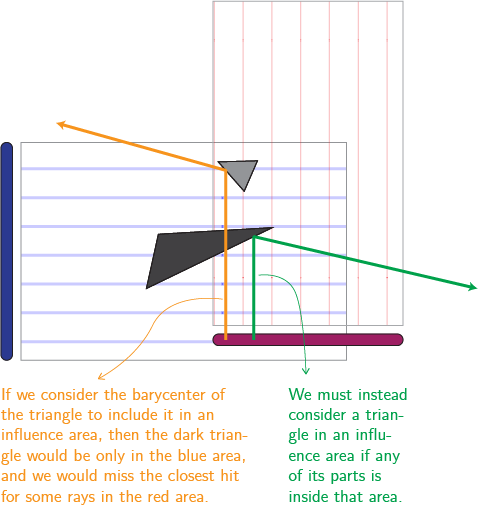
\includegraphics[width=\textwidth*\real{0.7}]{Images/double_area.png}
    \caption{Example of why it is necessary to use a conservative approach.}
    \label{fig:conservative_inside}
\end{figure}

Influence areas do not guarantee to cover the whole scene. It is indeed more frequent that regions of the scene don't have any particular ray distribuition. In this case, those triangles that are not inside any influence area, would not be part of any BVH, and would therefore be invisible to rays. For this very reason, it is necessary to build a global BVH for the whole scene. In our implementation, this BVH is built by using surface area heuristic.

When a ray traverses a local BVH and no hit is found, it is necessary to traverse the global BVH. It is indeed possible to find a hit with triangles that are not inside the influence area of the local BVH, as it can be observed in figure \ref{fig:outside_area}. However, if a ray is found in the local BVH, it is guaranteed for it to be the closest one, as shown in figure \ref{fig:conservative_inside}.

\begin{figure}[H]
    \centering
    \includegraphics[width=\textwidth*\real{0.7}]{Images/outside_area.png}
    \caption{Example of how it is possible that a hit is found in the global BVH, but not in the local one.}
    \label{fig:outside_area}
\end{figure}

\section{Top Level Structure} \label{sec:top_level_structure}
At the beginning of this chapter we stated that the first affinity criterion between a ray and an influence area is that the origin of the ray is inside the influence area. We have also seen how BVHs associated with influence areas contain only triangles that are inside the influence area. It is therefore of paramount importance to have a fast method to detect whether a point is inside a certain 3D region of the scene. 

In our implementation we tried to tackle this problem by using two different approaches. We will now briefly describe them from a theoretical point of view. All the details of our implementation can be found in section \ref{TODO}.

The first approach is to use algorithms described in appendices \ref{sec:point_inside_aabb} and \ref{sec:point_inside_frustum}. The complexity of this method linearly depends on the amount of influence areas present in the scene. Moreover, the algorithms to find out if a point is inside an OBB or a frustum are not cheap, especially in a scenario where they must be used for every single ray. On the other hand, all the influence areas can be easily stored in an array, therefore there is no overhead in building an ad-hoc structure.

On the opposite side of the spectrum there is the second method we propose. In this case we build an octree, where each leaf contains the influence areas that overlap with it. Building such an octree is not trivial, and it is diffusely described in section \ref{TODO}. However, once the octree is built, it is extremely cheap to find out what are the influence areas containing any given 3D point.

\chapter{Splitting Plane Facing Technique} \label{ch:splitting_plane_facing_technique}

\chapter{Implementation} \label{ch:implementation}

\chapter{Experimental Results} \label{ch:experimental_results}

\chapter{Use Cases} \label{ch:use_cases}

\chapter{Conclusion and Future Developments} \label{ch:conclusion}


% === Bibliography ===
\addtocontents{toc}{\vspace{2em}} % Add a gap in the Contents, for aesthetics
\bibliography{Bibliography} % The references information are stored in the file named "Bibliography.bib"


% === Appendices ===
\cleardoublepage
\addtocontents{toc}{\vspace{2em}} % Add a gap in the Contents, for aesthetics
\appendix

\chapter{Collision and Culling Algorithms}
\section{Ray-AABB Intersection} \label{sec:ray_box_intersection}
The algorithm we used to detect intersections between a ray and an AABB is the branchless slab algorithm \cite{ray_box_intersection}.

Given a ray in the form: $r(t) = O + t\cdot d$, where $O$ is the origin and $d$ the direction, the main idea of the algorithm is to find the 2 values of $t$ ($\overline{t_1}$ and $\overline{t_2}$) such that $r(\overline{t_{1,2}})$ are the points where the ray intersects the AABB.

Since the object to intersect the ray with is an axis-aligned bounding box in the min-max form, the algorithm can proceed one dimension at a time:
\begin{enumerate}
	\item First, it finds the intersection points of the ray with the planes parallel to the $yz$ plane, and sorts them in an ascending order with reference to the corresponding $\overline{t_{1,2}}$ values. We call the point with the smallest $\overline{t}$ value the \textit{closest}, and the other one the $\overline{furthest}$.
	\item Then it does the same with the $xz$ plane:
	\begin{itemize}
		\item As closest intersection point, it keeps the furthest between the 2 closest intersection points found so far (the one with the $yz$ plane and the one with the $xz$ plane).
		\item As furthest intersection point, it keeps the closest between the 2 furthest intersection points found so far.
	\end{itemize}
	\item Then it does the same with the $xy$ plane.
	\item Finally, an intersection is detected only in the case where the furthest intersection point actually has an associated $\overline{t}$ value bigger than the one of the closest point found by the algorithm.
	\item The returned $\overline{t}$ value is the smaller one, as long as it is greater or equal to 0; otherwise it means that the origin of the ray is inside the AABB, and one of the intersection points is \textit{behind} the ray origin.
\end{enumerate}
	
\begin{figure}[H]
    \centering
    \includegraphics[width=\textwidth]{Images/ray_aabb_intersection.png}
    \caption{Visual representation of the presented algorithm in 2 dimensions. An interactive simulation of this algorithm can be found at: \url{https://www.geogebra.org/m/np3tnjvb}.}
    \label{fig:ray_aabb_intersection}
\end{figure}

\begin{algorithm}[H]
	\caption{Ray-AABB branchless slab intersection algorithm in 3 dimensions}
	\begin{algorithmic}[1]
		\Function{Intersect}{$ray, aabb$}
		\Let {$t1_x$}{$\frac{aabb.min.x - ray.origin.x}{ray.direction.x}$} \Comment{yz plane}
		\Let {$t2_x$}{$\frac{aabb.max.x - ray.origin.x}{ray.direction.x}$}
		\Let {$tMin$}{$min(t1_x, t2_x)$}
		\Let {$tMax$}{$max(t1_x, t2_x)$}
		\Let {$t1_y$}{$\frac{aabb.min.y - ray.origin.y}{ray.direction.y}$} \Comment{xz plane}
		\Let {$t2_y$}{$\frac{aabb.max.y - ray.origin.y}{ray.direction.y}$}
		\Let {$tMin$}{$ max(tMin, min(t1_y, t2_y))$}
		\Let {$tMax$}{$ min(tMax, max(t1_y, t2_y))$}
		\Let {$t1_z$}{$\frac{aabb.min.z - ray.origin.z}{ray.direction.z}$} \Comment{xy plane}
		\Let {$t2_z$}{$\frac{aabb.max.z - ray.origin.z}{ray.direction.z}$}
		\Let {$tMin$}{$max(tMin, min(t1_z, t2_z))$}
		\Let {$tMax$}{$min(tMax, max(t1_z, t2_z))$}
		\Let {$areColliding$}{$tMax > tMin$ \AAnd $tMax \geq 0$}
		\Let {$collisionDist$}{$tMin < 0 \: ? \: tMax \: : \: tMin$}
		\State \Return $\langle areColliding, collisionDist \rangle$
		\EndFunction
	\end{algorithmic}
\end{algorithm} 

It is interesting to note how, under the floating-point IEEE 754 standard, the algorithm also works when it is not possible to find an intersection point along a certain axis (i.e. when the ray is parallel to certain planes). Indeed, in such cases, the values $\overline{t_{1,2}}$ will be $\pm \infty$, and the comparisons will still be well defined.

\section{Ray-Plane Intersection} \label{sec:ray_plane_intersection}
For ray-plane intersection we decided to use this algorithm presented in the educational portal of the SIGGRAPH conference \cite{ray_plane_intersection}.

Given a ray in the form: $r(t) = O + t\cdot d$, where $O$ is the origin and $d$ the direction, and a plane whose normal $n$ and a point $P$ are known, we first check whether the plane and the ray are parallel, in which case no intersection can be found.

Then, if they are not parallel, we obtain the analytic form of the 3-dimensional plane: 
\begin{align*}
	A\cdot x + B\cdot y + C\cdot z + D = 0
\end{align*}
In particular, we know a point $P$ that is part of the plane, therefore we can obtain the $D$ parameter:
\begin{align*}
&A\cdot P_x + B\cdot P_y + C\cdot P_z + D = 0\\
\implies& D = -(A\cdot P_x + B\cdot P_y + C\cdot P_z)
\end{align*}
By definition, the vector formed by the parameters $[A,B,C]$ is perpendicular to the plane, therefore:
\begin{align*}
&D = -(n_x\cdot P_x + n_y\cdot P_y + n_z\cdot P_z)\\
\implies& D = -\langle n \cdot P \rangle
\end{align*}
Now that we have the parametric equation of the plane, we can force a point of the plane to also be a point of the ray: 
\begin{align*}
	&A\cdot r(t)_x + B\cdot r(t)_y + C\cdot r(t)_z + D = 0\\
	\implies& A\cdot (O_x + t\cdot d_x) + B\cdot (O_y + t\cdot d_y) + C\cdot (O_z + t\cdot d_z) + D = 0\\
	\implies& t = \frac{-\langle n\cdot O \rangle + D}{\langle n\cdot d \rangle}
\end{align*}
Finally, if the found $\overline{t}$ value is negative, it means that the intersection point between the ray and the plane is \textit{behind} the ray origin, therefore no intersection is found. Else the ray intersects the plane at point $r(\overline{t})$.

\begin{algorithm}[H]
	\caption{Ray-plane intersection algorithm}
	\begin{algorithmic}[1]
		\Function{Intersect}{$ray, plane$}
		\Let{$d$}{$ray.direction$}
		\Let{$O$}{$ray.origin$}
		\Let{$n$}{$plane.normal$}
		\Let{$P$}{$plane.point$}
		\If{$\langle n\cdot d \rangle = 0$} \Comment{Ray is parallel to plane}
			\State \Return $\langle false, \_ \rangle$
		\EndIf
		\Let{$D$}{$-\langle n\cdot P \rangle$}
		\Let{$t$}{$\frac{-\langle n\cdot O \rangle}{\langle n\cdot d \rangle}$}
		\If{$t<0$} \Comment{Intersection point is \textit{behind} ray origin}
			\State \Return $\langle false, \_ \rangle$
		\Else
			\State \Return $\langle true, t \rangle$
		\EndIf
		\EndFunction
	\end{algorithmic}
\end{algorithm} 

\section{Ray-Triangle Intersection} \label{sec:ray_triangle_intersection}
Once we have algorithms to check for ray-plane intersection (\ref{sec:ray_plane_intersection}) and for a point inside a 2D convex hull (\ref{sec:point_inside_2dHull}), we can combine them to check if a ray intersects a triangle and to compute the coordinates of the intersection point:

\begin{enumerate}
	\item Build a plane that has as normal the normal to the triangle, and as point any vertex of the triangle;
	\item Use the ray-plane intersection algorithm (\ref{sec:ray_plane_intersection}) to find the coordinates of the point where the ray and the plane collide (if any);
	\item Use the point inside 2D convex hull test (\ref{sec:point_inside_2dHull}) to determine if the intersection point is inside the triangle.
\end{enumerate}

\section{AABB-AABB Intersection} \label{sec:aabb_aabb_intersection}
To detect a collision between 2 axis-aligned bounding boxes in the min-max form, it is sufficient to check that there is an overlap between them in all 3 dimensions. By naming the 2 AABBs as $A$ and $B$ we get:
\begin{subequations}
	\begin{align*}[left=\empheqlbrace]
		A.min_x \leq& B.max_x \\
		A.max_x \geq& B.min_x \\
		A.min_y \leq& B.max_y \\
		A.max_y \geq& B.min_y \\
		A.min_z \leq& B.max_z \\
		A.max_z \geq& B.min_z
	\end{align*}
\end{subequations}

\section{Frustum-AABB Intersection} \label{sec:frustum_aabb_intersection}
In order to detect an intersection between a frustum and an axis-aligned bounding box in the min-max form, we used a simplified version of the separating axis test (a special case of the separating hyperplane theorem) \cite{separating_axis_test}. The simplification comes from the fact that we need to find the intersection of a frustum and an AABB, and not two 3D convex hulls, meaning that we can exploit some assumptions on the direction of the edges of the two objects, as we'll note below.

Before proceeding with the separating axis test, we first try a simpler AABB-AABB collision test, between the given AABB and the AABB that most tightly encloses the frustum. In case this \textit{rejection test} gives a negative answer, we can deduce that the frustum and the AABB are not colliding. Otherwise, we must use the more expensive SAT.

The separating axis theorem in 3 dimensions states that 2 convex hulls are not colliding if and only if there is a plane that divides the space into 2 half-spaces each fully containing one of the two convex hulls.\\
To find whether such a plane exists, we project the two convex hulls on certain axes, and check whether their 1D projections are overlapping. The theorem also states that if there is an axis where the projections are not overlapping it must be either:
\begin{itemize}
	\item An axis perpendicular to one of the faces of the convex hulls, or
	\item An axis parallel to the cross product between an edge of the first convex hull and an edge of the second convex hull.
\end{itemize}
This consideration makes it possible to use the theorem in a concrete scenario.

\begin{figure}[H]
    \centering
    \includegraphics[scale=0.35]{Images/aabb_1d_proj.png} 
    \caption{The projection of an AABB on an axis.}
    \label{fig:aabb_1d_proj}
\end{figure}

In principle, given 2 polyhedra with 6 faces each (such as a frustum and an AABB), there should be $(6 + 6)_{normals} + (12\cdot 12)_{cross\: products} = 156$ axis to check; but, since:
\begin{itemize}
	\item The AABB has edges only in 3 different directions, and faces normals only in 3 different directions, and
	\item The frustum has edges only in 6 different directions, and faces normals only in 5 different directions
\end{itemize}
the number of checks is reduced to $(3 + 5)_{normals} + (3\cdot 6)_{cross\: products} = 26$.

\begin{figure}[H]
    \centering
    \subfloat[AABB: 3 different edges directions]{
        \includegraphics[scale=0.35]{Images/aabb_edges_same_dir.png}
		}
		\qquad
	\subfloat[Frustum: 6 different edges directions]{
        \includegraphics[scale=0.35]{Images/frustum_edges_same_dir.png}
    }
	\caption{In the figure the edges having the same direction are colored in the same color.}
    \label{fig:aabb_frustum_different_edges_directions}
\end{figure}


\subsection{1D Projections Overlapping Test}
In order to detect if the 1D projections of the 3D hulls are overlapping, we identify the outermost points of each projection (namely $A_{min}, A_{max}, B_{min}, B_{max}$) and check that $B_{min} \leq A_{max} \And B_{max} \geq A_{min}$.\\
For the AABB another optimization is possible, where we detect what points will be the outermost after the projection without actually projecting them, based on the direction of the axis:

\begin{figure}[H]
    \centering
    \subfloat[AABB vertices layout.]{
        \raisebox{-0.1\height}{\includegraphics[scale=0.35]{Images/aabb.png}}
    }
    \quad
    \subfloat{
		\raisebox{0.5\height}{
		\begin{tabular}{| c | c |}
			\hline
			\textbf{axis direction} & \textbf{extremes} \\
			\hline \hline
			$x \geq 0 \And y \geq 0 \And z \leq 0$ & 1, 6\\
			$x \leq 0 \And y \leq 0 \And z \geq 0$ & 6, 1\\
			$x \geq 0 \And y \geq 0 \And z \geq 0$ & 0, 7\\
			$x \leq 0 \And y \leq 0 \And z \leq 0$ & 7, 0\\
			$x \geq 0 \And y \leq 0 \And z \leq 0$ & 3, 4\\
			$x \leq 0 \And y \geq 0 \And z \geq 0$ & 4, 3\\
			$x \geq 0 \And y \leq 0 \And z \geq 0$ & 2, 5\\
			$x \leq 0 \And y \geq 0 \And z \leq 0$ & 5, 2\\
			\hline
		\end{tabular}
		}
    }
    \label{fig:aabb_projected_extremes}
\end{figure}

\begin{algorithm}[H]
	\caption{Ray-AABB branchless slab intersection algorithm in 3 dimensions}
	\begin{algorithmic}[1]
		\Function{Intersect}{$frustum, aabb$}
		\If{$!intersect(frustum.aabb, aabb)$} \Comment{AABB-AABB test}
			\State \Return $false$
		\EndIf
		\Let{$axesToCheck$}{$(\perp frustum \: faces) \cup (\perp AABB \: faces) \cup (\times edges$)}
		\ForAll{$axis \in axesToCheck$}
			\Let{$frustumExtremes$}{$findFrustumExtremes(frustum, axis)$} \Comment{Returns the vertices of the frustum that, after the projection, will be the extremes}
			\Let{$aabbExtremes$}{$findAabbExtremes(aabb, axis)$} \Comment{Same as above, but uses the discussed optimization}
			\Let{$A_{min}$}{$\langle aabbExtremes.first \cdot axis \rangle$}
			\Let{$A_{max}$}{$\langle aabbExtremes.second \cdot axis \rangle$}
			\Let{$B_{min}$}{$\langle frustumExtremes.first \cdot axis \rangle$}
			\Let{$B_{max}$}{$\langle frustumExtremes.second \cdot axis \rangle$}
			\If{$!(B_{min} \leq A_{max} \And B_{max} \geq A_{min})$} 
				\State \Return $false$
			\EndIf
		\EndFor
		\State \Return $true$ \Comment{If we havent't found any axis where there is no overlap, boxes are colliding}
		\EndFunction
	\end{algorithmic}
\end{algorithm} 

\section{Point inside AABB Test} \label{sec:point_inside_aabb}
To check if a point $P$ is inside an axis-aligned bounding box in the min-max form, it is sufficient to compare its coordinates with the minimum and maximum of the AABB component-wise:
\begin{subequations}
	\begin{align*}[left=\empheqlbrace]
		min_x \leq P_x \leq max_x \\
		min_y \leq P_y \leq max_y \\
		min_z \leq P_z \leq max_z
	\end{align*}
\end{subequations}

\section{Point inside Frustum Test} \label{sec:point_inside_frustum}
It is possible to detect whether a point is inside a 3-dimensional frustum by projecting it with the perspective matrix associated with the frustum and then comparing its coordinates, as suggested by \cite{point_inside_frustum_test}.

Given the perspective matrix $\textit{M}$ associated with the frustum, we can project a point $P$ and get: $P' = \textit{M} \cdot P$; and perform the perspective division. 

$P'' = \frac{P'}{P'_w}$ $P''$ is now in normalized device coordinates (NDC) space, where the frustum is an axis-aligned bounding box that extends from $\langle -1, -1, -1 \rangle$ to $\langle 1, 1, 1 \rangle$ \footnote{Based on the convention used, it is possible that the AABB in NDC space has a different size. For example, it is common an AABB extending from $\langle -1, -1, 0 \rangle$ to $\langle 1, 1, 1 \rangle$}.

It is now immediate to see that $P$ is inside the frustum if and only if $P''$ is inside the AABB (see section \ref{sec:point_inside_aabb}).

A simple optimization allow us to avoid the perspective division. Indeed, since in homogeneous coordinates:
$$\langle x',y',z',w' \rangle = \langle \frac{x'}{w'},\frac{y'}{w'},\frac{z'}{w'},\frac{w'}{w'} \rangle = \langle x'',y'',z'',1 \rangle$$
We can change the inequalities to check whether the point is inside the frustum from:

\begin{minipage}{.4\linewidth}
	\begin{subequations}
		\begin{align*}[left=\empheqlbrace]
			-1 \leq x'' \leq 1 \\
			-1 \leq y'' \leq 1 \\
			-1 \leq z'' \leq 1
		\end{align*}
	\end{subequations}
\end{minipage}
		to:
\begin{minipage}{.4\linewidth}
	\begin{subequations}
		\begin{align*}[left=\empheqlbrace]
			-w' \leq x' \leq w' \\
			-w' \leq y' \leq w' \\
			-w' \leq z' \leq w'
		\end{align*}
	\end{subequations}
\end{minipage}

We created a 2D visual demonstration of how it is possible to detect if a point is inside a frustum at \url{https://www.geogebra.org/m/ammj5mxd}.

\section{Point inside 2D Convex Hull Test} \label{sec:point_inside_2dHull}
Given a 2D convex hull in 3-dimensional space and a 3D point laying on the same plane as the hull, it is possible to use a simple inside-outside test \cite{ray_triangle_intersection} to determine whether the point is inside the convex hull.

The main idea is that the point lays inside the convex hull if and only if it is \textit{to the right} (or \textit{to the left}, depending on the winding order) of all the edges of the hull.

In order to determine the relative position of a point and an edge $\overline{AB}$, we can look at the cross product:
$$u \times v \; where \; u = \overrightarrow{AB}, v = \overrightarrow{AP}$$

\begin{figure}[H]
    \centering
    \includegraphics[scale=0.4]{Images/cross_product.png} 
    \caption{Visualization of cross product.}
    \label{fig:cross_product}
\end{figure}

Therefore the strategy to determine if a point is on the same side of all the edges of the convex hull is to compute a reference cross product, by choosing any of the edges, and then making sure that all the other cross products have the same direction. To check that 2 vectors have the same direction it is sufficient that their dot product is positive.

\begin{algorithm}[H]
	\caption{Inside-outside test between a 3D point and a 2D convex hull.} 
	\begin{algorithmic}[1]
		\Function{IsInside}{$P, hull$}
		\Let{$N$}{$number \: of \: edges \: of \: hull$}
		\Let{$u$}{$hull[0] - hull[N-1]$}
		\Let{$v$}{$P - hull[N-1]$}
		\Let{$ref$}{$u \times v$} \Comment{The reference cross product}
		\For{$0\leq i < N$}
			\Let{$u$}{$hull[i+1] - hull[i]$}
			\Let{$v$}{$P - hull[i]$}
			\Let{$cross$}{$u \times v$}
			\If{$\langle ref \cdot cross \rangle \leq 0$}
				\State \Return $false$
			\EndIf
		\EndFor
		\State \Return $true$
		\EndFunction
	\end{algorithmic}
\end{algorithm} 

\section{2D Convex Hull Culling} \label{sec:2dHull_culling}
In order to find the overlapping region between two 2D hulls in 2-dimensional space, we can proceed as illustrated in the diagram below (\cite{convex_hull_culling}):

\begin{figure}[H]
    \centering
    \includegraphics[scale=0.7]{Images/hull_culling.png} 
    \caption{General algorithm to find the overlapping region between two convex hulls called $A$ and $B$.}
    \label{fig:hull_culling}
\end{figure}

\begin{figure}[H]
    \centering
    \includegraphics[scale=0.4]{Images/overlapping_hull.png} 
    \caption{Yellow vertices are found in the first 2 steps (vertices inside), whereas light blue vertices are found in the third step (edges intersections).}
    \label{fig:overlapping_hull}
\end{figure}

We'll now go through each phase and see the used algorithms.

\subsection{Vertices inside convex hull}
To find out what vertices of a hull are inside the other one we simply looped over them and used the point inside convex hull test (\ref{sec:point_inside_2dHull}).

\subsection{Edges intersections}
To detect an intersection between two segments, we first have to compute the equation of the line the segment is lying on.

Given a segment $\overline{PQ}$, the underlying line has equation:
$$A\cdot x + B\cdot y = C$$
We can then compute the parameters of the line as:
\begin{subequations}
	\begin{align*}[left=\empheqlbrace]
		A &= Q_y - P_y\\
		B &= P_x - Q_x\\
		C &= A\cdot P_x + B\cdot P_y
	\end{align*}
\end{subequations}

After we calculate the underlying line of both segments, with parameters $A_1, B_1, C_1, A_2, B_2, C_2$, we can compute the intersection point $K$ of the two lines as:
\begin{subequations}
	\begin{align*}[left=\empheqlbrace]
		\Delta &= A_1 \cdot B_2 - A_2 \cdot B_1\\
		K_x &= \frac{B_2 \cdot C_1 - B_1 \cdot C_2}{\Delta}\\
		K_y &= \frac{A_1 \cdot C_2 - A_2 \cdot C_1}{\Delta}
	\end{align*}
\end{subequations}

We are now left with the task of verifying whether the found intersection point $K$ is in between both segments' extremes. Let's call the first segment $\overline{MN}$ and the second one $\overline{PQ}$:

\begin{minipage}{.4\linewidth}
	\begin{subequations}
		\begin{align*}[left=\empheqlbrace]
			min(M_x, N_x) &\leq K_x \And\\
			max(M_x, N_x) &\geq K_x \And\\
			min(M_y, N_y) &\leq K_y \And\\
			max(M_y, N_y) &\geq K_y		
		\end{align*}
	\end{subequations}
\end{minipage}
		$And$
\begin{minipage}{.4\linewidth}
	\begin{subequations}
		\begin{align*}[left=\empheqlbrace]
			min(P_x, Q_x) &\leq K_x \And\\
			max(P_x, Q_x) &\geq K_x \And\\
			min(P_y, Q_y) &\leq K_y \And\\
			max(P_y, Q_y) &\geq K_y		
		\end{align*}
	\end{subequations}
\end{minipage}

\begin{figure}[H]
    \centering
    \includegraphics[scale=0.4]{Images/segments_intersection.png} 
    \caption{In this example segments do not collide because $max(M_x, N_x) = N_x \ngeq K_x$ or $max(M_y, N_y) \ngeq K_y$}
    \label{fig:segments:intersection}
\end{figure}

\subsection{Vertices ordering}
Given a set of unordered 2D points belonging to a convex hull, we want to sort them in a counterclockwise order, so that two consecutive vertices form an edge of the convex hull.

To do so we can compute the barycenter $O$ of the set of points that, being them part of a convex hull\footnote{We can state that the vertices we found so far make up a convex hull because the overlapping of two convex hulls is necessarily a convex hull.}, is necessarily inside the convex hull itself.

Now, for each vertex $A_k$ we can calculate the vector $\overrightarrow{OA_k}$, and sort the vertices based on $atan2(\overrightarrow{OA_k}_y, \overrightarrow{OA_K}_x)$.

The $atan2(v_y, v_x)$ function returns the angle between the positive x-axis and the vector $v=\langle v_x, v_y \rangle$. Differently from the arctangent function, the returned angle ranges in the interval $(-\pi, \pi]$, therefore is well suited for our purpose of sorting the convex hull vertices.

\begin{figure}[H]
    \centering
    \includegraphics[scale=0.4]{Images/vertices_sorting.png} 
    \caption{Vertices of a convex hull before and after $atan2$ sorting.}
    \label{fig:vertices_sorting}
\end{figure}

\section{2D Hull Area Computation} \label{sec:2dHull_area_computation}
To calculate the area of a 2-dimensional hull we decided to use the Gauss's area formula, also known as the shoelace formula \cite{shoelace_formula}.

Given a polygon with vertices $P_0, P_1, ..., P_n$, where each vertex has coordinates: $P_k = (x_k, y_k)$, its area can be found with this formula:
\begin{align*}
	Area =& \bigg|\frac{1}{2}\cdot\left(\begin{vmatrix} x_0 & y_1\\y_0 & y_1 \end{vmatrix} + \begin{vmatrix} x_1 & y_2\\y_1 & y_2 \end{vmatrix} + ... + \begin{vmatrix} x_{n-1} & y_n\\y_{n-1} & y_n \end{vmatrix} + \begin{vmatrix} x_n & y_0\\y_n & y_0 \end{vmatrix}\right)\bigg|\\
	=& \Bigg|\frac{\displaystyle\sum_{i=0}^{n}(x_i \cdot y_{i+1} - y_i \cdot x_{i+1})}{2}\Bigg|
\end{align*}

In the last formula we consider $P_0 = P_{n+1}$.

\chapter{Multiple Importance Sampling} \label{ch:mis}
TODO

% === Lists ===
\listoffigures
\listoftables

% Table of symbols


\chapter*{List of Symbols} % You have to include a chapter for your list of symbols (
\begin{table}[H]
    \centering
    \begin{tabular}{lll}
        \textbf{Symbol} & \textbf{Description} & \textbf{Unit} \\\hline\\[-9px]
        $\bm{alpha}$ & symbol 1 & km \\[2px]
    \end{tabular}
\end{table}

% === Ringraziamenti ===
\chapter*{Ringraziamenti}
\small
Lorem ipsum dolor sit amet, consectetur adipiscing elit, sed do eiusmod tempor incididunt ut labore et dolore magna aliqua. Ultricies integer quis auctor elit sed vulputate mi. Accumsan sit amet nulla facilisi morbi. Suspendisse potenti nullam ac tortor vitae purus faucibus. Ultricies lacus sed turpis tincidunt id. Sit amet mauris commodo quis imperdiet. Arcu bibendum at varius vel. Venenatis urna cursus eget nunc. Mus mauris vitae ultricies leo integer malesuada nunc vel. Sodales neque sodales ut etiam sit. Pellentesque dignissim enim sit amet venenatis urna cursus eget nunc. Condimentum mattis pellentesque id nibh tortor id aliquet lectus. Ultrices gravida dictum fusce ut placerat orci nulla pellentesque dignissim. Faucibus pulvinar elementum integer enim neque. Morbi tincidunt augue interdum velit euismod in pellentesque massa.

A diam maecenas sed enim ut sem viverra aliquet eget. Viverra aliquet eget sit amet tellus cras. Tellus at urna condimentum mattis pellentesque. Quis viverra nibh cras pulvinar. Posuere morbi leo urna molestie at elementum. Aenean euismod elementum nisi quis eleifend quam. In hac habitasse platea dictumst vestibulum rhoncus. Nullam non nisi est sit amet facilisis magna etiam tempor. Neque laoreet suspendisse interdum consectetur libero. Vitae auctor eu augue ut lectus arcu bibendum. Ipsum consequat nisl vel pretium lectus quam. Velit dignissim sodales ut eu sem. Odio morbi quis commodo odio. Lectus nulla at volutpat diam. Neque gravida in fermentum et sollicitudin ac. Nunc non blandit massa enim nec dui nunc. Quisque id diam vel quam elementum pulvinar etiam non quam. Consequat id porta nibh venenatis cras sed felis. Vitae justo eget magna fermentum iaculis eu non diam. Mi sit amet mauris commodo.
\normalsize

\ClearShipoutPicture

\triangleLogo
\end{document}
